\documentclass{beamer}\usepackage[]{graphicx}\usepackage[]{color}
%% maxwidth is the original width if it is less than linewidth
%% otherwise use linewidth (to make sure the graphics do not exceed the margin)
\makeatletter
\def\maxwidth{ %
  \ifdim\Gin@nat@width>\linewidth
    \linewidth
  \else
    \Gin@nat@width
  \fi
}
\makeatother

\definecolor{fgcolor}{rgb}{0.345, 0.345, 0.345}
\newcommand{\hlnum}[1]{\textcolor[rgb]{0.686,0.059,0.569}{#1}}%
\newcommand{\hlstr}[1]{\textcolor[rgb]{0.192,0.494,0.8}{#1}}%
\newcommand{\hlcom}[1]{\textcolor[rgb]{0.678,0.584,0.686}{\textit{#1}}}%
\newcommand{\hlopt}[1]{\textcolor[rgb]{0,0,0}{#1}}%
\newcommand{\hlstd}[1]{\textcolor[rgb]{0.345,0.345,0.345}{#1}}%
\newcommand{\hlkwa}[1]{\textcolor[rgb]{0.161,0.373,0.58}{\textbf{#1}}}%
\newcommand{\hlkwb}[1]{\textcolor[rgb]{0.69,0.353,0.396}{#1}}%
\newcommand{\hlkwc}[1]{\textcolor[rgb]{0.333,0.667,0.333}{#1}}%
\newcommand{\hlkwd}[1]{\textcolor[rgb]{0.737,0.353,0.396}{\textbf{#1}}}%

\usepackage{framed}
\makeatletter
\newenvironment{kframe}{%
 \def\at@end@of@kframe{}%
 \ifinner\ifhmode%
  \def\at@end@of@kframe{\end{minipage}}%
  \begin{minipage}{\columnwidth}%
 \fi\fi%
 \def\FrameCommand##1{\hskip\@totalleftmargin \hskip-\fboxsep
 \colorbox{shadecolor}{##1}\hskip-\fboxsep
     % There is no \\@totalrightmargin, so:
     \hskip-\linewidth \hskip-\@totalleftmargin \hskip\columnwidth}%
 \MakeFramed {\advance\hsize-\width
   \@totalleftmargin\z@ \linewidth\hsize
   \@setminipage}}%
 {\par\unskip\endMakeFramed%
 \at@end@of@kframe}
\makeatother

\definecolor{shadecolor}{rgb}{.97, .97, .97}
\definecolor{messagecolor}{rgb}{0, 0, 0}
\definecolor{warningcolor}{rgb}{1, 0, 1}
\definecolor{errorcolor}{rgb}{1, 0, 0}
\newenvironment{knitrout}{}{} % an empty environment to be redefined in TeX

\usepackage{alltt}
\usefonttheme[onlymath]{serif}

\usepackage[portuguese]{babel}
\usepackage{graphicx}
\usepackage{ulem} % Para texto em strikeout
\usepackage{amsmath}
\usepackage{amssymb}

\usetheme{m}

\ifdefined\knitrout 
\renewenvironment{knitrout}{\setlength{\topsep}{0mm}}{}
\else
\fi

\title{Aula 5: Modelos Lineares Gerais II}
\subtitle{Análise Estatística e Modelagem de Dados Ecológicos}
\author{\textbf{Thiago S. F. Silva} - tsfsilva@rc.unesp.br}
\institute{Programa de Pós Graduação em Ecologia e Biodiversidade - UNESP}
\date{\today}

\graphicspath{{C:/Users/thiago/OneDrive/UNESP/Pos_graduacao/Eco/2015/Estatistica_2015/Aulas/Aula_5_Regressao_II/figuras/}}
\IfFileExists{upquote.sty}{\usepackage{upquote}}{}
\begin{document}



%===============================================================================%
\begin{frame}[plain] % plain avoids a badbox error from page number in title page
  \titlepage
\end{frame}

\begin{frame}{Outline}
  \tableofcontents
\end{frame}
%===============================================================================%

\section{Inferências sobre o modelo}


%===============================================================================%
\begin{frame}{Recapitulando: Regressão Linear Simples}

Quais os componentes de um modelo de regressão simples, estimado a partir de uma amostra de duas variáveis $X$ e $Y$?
\vfill
\centering
\only<2-3> {$\alert{\hat Y_i}$}
\only<4-5> {$\hat Y_i = \alert{b_0}$}
\only<6-7> {$\hat Y_i = b_0 + \alert{b_1}$}
\only<8-9> {$\hat Y_i = b_0 + b_1\alert{X_i}$}
\only<10-11> {$\hat Y_i = b_0 + b_1X_i + \alert{e_i}$}

\vfill

\only<3> {Estimador para o valor médio ($E[Y_i]$) da variável \textbf{dependente} $Y_i$}
\only<5> {Estimador do coeficiente \textbf{intercepto} ($\beta _0$), nos dá valor de $\hat Y_i$ quando $X_i=0$}
\only<7> {Estimador do coeficiente de \textbf{inclinação} ($\beta _1$), nos diz o quanto $\hat Y$ cresce/diminui quando $\Delta X=1$}
\only<9> {Variável \textbf{independente} ou \textbf{preditora}}
\only<11> {Resíduo de $\hat Y_i$, dado por $Y_i - \hat Y_i$, é um estimador dos erros da regressão, $\varepsilon$}


\end{frame}
%===============================================================================%


%===============================================================================%
\begin{frame}{Recapitulando: Regressão Linear Simples}

O que nós sabemos sobre os resíduos $e$? \pause
\vfill
\begin{itemize}
  \item Possuem média zero, $E(e) = 0$ \pause
  \item Possuem variância constante, $Var(e) = s^2$ \pause
\end{itemize}  
\vfill
O que nós sabemos sobre $\hat Y$? \pause
\vfill
\begin{itemize}
  \item Sua média é dada pela equação da reta, $E(\hat Y) = b_0 + b_1X$ \pause
  \item Também possuem variância constante, já que $Var(\hat Y) = Var(e) = s^2$
\end{itemize}  

\end{frame}
%===============================================================================%


%===============================================================================%
\begin{frame}{Recapitulando: Regressão Linear Simples}

O que nós sabemos sobre $b_0$ e $b_1$? \pause
\vfill
\begin{itemize}
  \item São estimados pelo método dos Mínimos Quadrados (\emph{Least Squares}) \pause
  \item São os melhores estmadores para $\beta _0$ e $\beta_1$: \pause
  \begin{itemize}
    \item São estimadores não-tendenciosos \pause
    \item Possuem a menor variância possível dentre todos os estimadores \pause  
    \end{itemize}
\end{itemize}  
\vfill
O que nós \alert{\textbf{não}} sabemos sobre $\hat Y$,$b_0$, $b_1$ e $e$? \pause
\vfill
\begin{itemize}
  \item $\hat Y \sim ?(b_0 + b_1X,s^2)$ \pause
  \item $b_0 \sim ?(b_0,?)$; $b_1 \sim ?(b_1,?)$ \pause
  \item $e \sim ?(0,s^2)$
\end{itemize}  
\vfill

\end{frame}
%===============================================================================%


%===============================================================================%
\begin{frame}{Recapitulando: Regressão Linear Simples}

\textbf{Fato interessante (e importante):}
\vfill
O método dos Mínimos Quadrados \textbf{garante} que $b_0$ e $b_1$ são os \textbf{melhores} estimadores de $\beta _0$ e $\beta _1$, \textbf{qualquer que seja} a distribuição de $\varepsilon$ \pause
\vfill
Isso significa que, independentemente da distribuição dos resíduos (e de $Y$), a reta de regressão é o melhor estimador para $E(Y)$
\end{frame}
%===============================================================================%

%===============================================================================%
\begin{frame}[fragile]
\begin{columns}[b]

\column{0.5\linewidth}

\begin{knitrout}\tiny
\definecolor{shadecolor}{rgb}{0.969, 0.969, 0.969}\color{fgcolor}\begin{kframe}
\begin{alltt}
\hlkwd{set.seed}\hlstd{(}\hlnum{511}\hlstd{)}
\hlstd{x1} \hlkwb{<-} \hlkwd{c}\hlstd{(}\hlnum{0}\hlopt{:}\hlnum{50}\hlstd{)}
\hlstd{y1} \hlkwb{<-} \hlnum{2} \hlopt{+} \hlnum{3}\hlopt{*}\hlstd{x1} \hlopt{+} \hlkwd{rnorm}\hlstd{(}\hlnum{51}\hlstd{,}\hlnum{0}\hlstd{,}\hlnum{5}\hlstd{)}
\hlstd{m1} \hlkwb{<-} \hlkwd{lm}\hlstd{(y1} \hlopt{~} \hlstd{x1)}
\hlkwd{plot}\hlstd{(x1,y1)}
\hlkwd{abline}\hlstd{(m1)}
\hlkwd{hist}\hlstd{(m1}\hlopt{$}\hlstd{residuals,}\hlkwc{breaks}\hlstd{=}\hlnum{30}\hlstd{,}\hlkwc{main}\hlstd{=}\hlnum{NA}\hlstd{)}
\end{alltt}
\end{kframe}
\end{knitrout}

\column{0.5\linewidth}

\begin{knitrout}
\definecolor{shadecolor}{rgb}{0.969, 0.969, 0.969}\color{fgcolor}
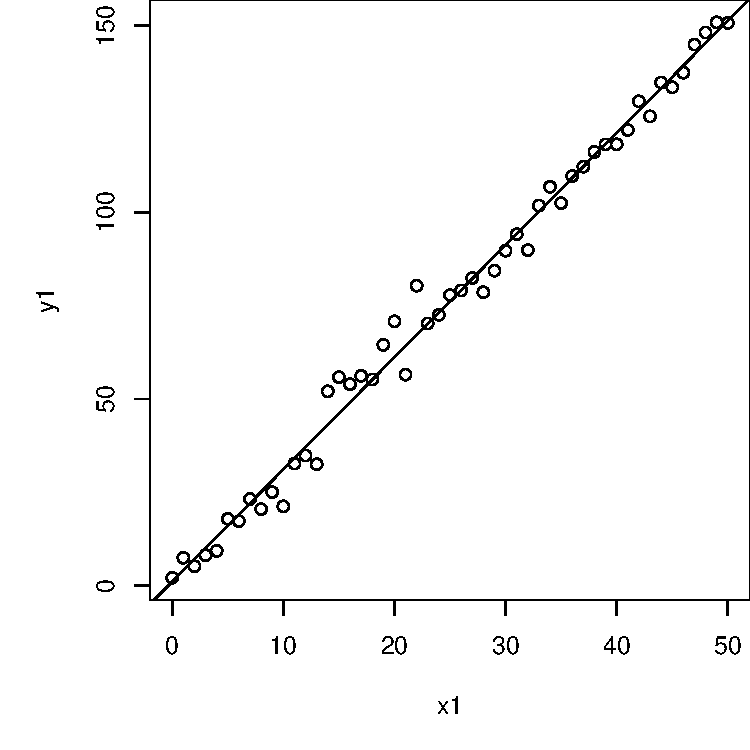
\includegraphics[width=0.8\linewidth]{figure/unnamed-chunk-2-1} 

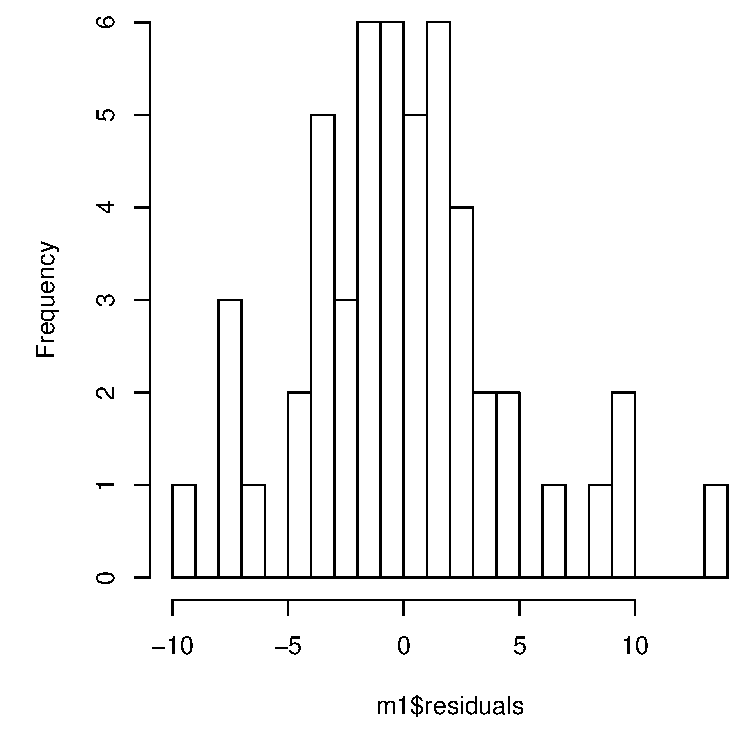
\includegraphics[width=0.8\linewidth]{figure/unnamed-chunk-2-2} 

\end{knitrout}

\end{columns}

\end{frame}
%===============================================================================%

%===============================================================================%
\begin{frame}[fragile]
\begin{columns}[b]

\column{0.5\linewidth}

\begin{knitrout}\tiny
\definecolor{shadecolor}{rgb}{0.969, 0.969, 0.969}\color{fgcolor}\begin{kframe}
\begin{alltt}
\hlkwd{set.seed}\hlstd{(}\hlnum{511}\hlstd{)}
\hlstd{x2} \hlkwb{<-} \hlkwd{c}\hlstd{(}\hlnum{0}\hlopt{:}\hlnum{50}\hlstd{)}
\hlstd{y2} \hlkwb{<-} \hlnum{2} \hlopt{+} \hlnum{3}\hlopt{*}\hlstd{x2} \hlopt{+} \hlkwd{rexp}\hlstd{(}\hlnum{51}\hlstd{,}\hlnum{0.2}\hlstd{)}
\hlstd{m2} \hlkwb{<-} \hlkwd{lm}\hlstd{(y2} \hlopt{~} \hlstd{x2)}
\hlkwd{plot}\hlstd{(x2,y2)}
\hlkwd{abline}\hlstd{(m2)}
\hlkwd{hist}\hlstd{(m2}\hlopt{$}\hlstd{residuals,}\hlkwc{breaks}\hlstd{=}\hlnum{30}\hlstd{,}\hlkwc{main}\hlstd{=}\hlnum{NA}\hlstd{)}
\end{alltt}
\end{kframe}
\end{knitrout}

\column{0.5\linewidth}

\begin{knitrout}
\definecolor{shadecolor}{rgb}{0.969, 0.969, 0.969}\color{fgcolor}
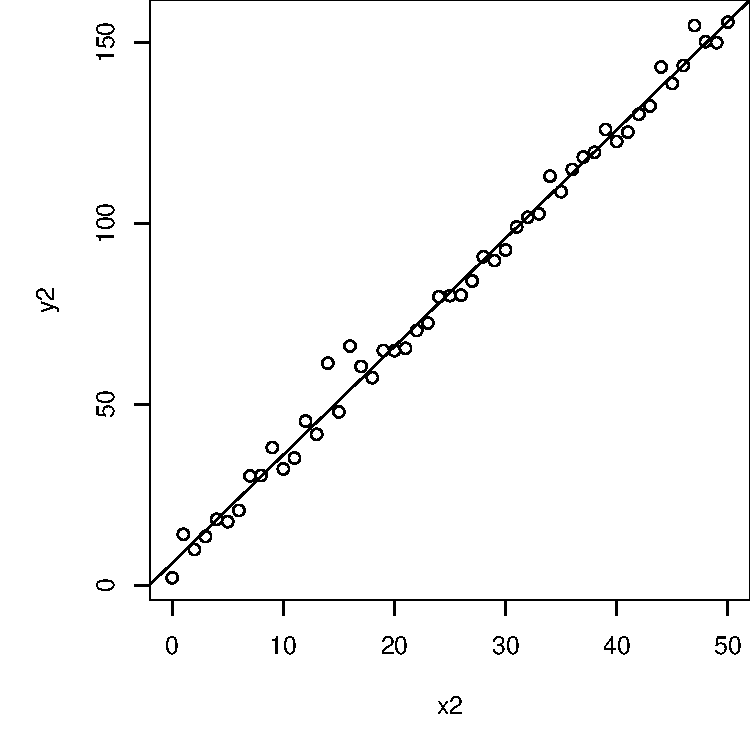
\includegraphics[width=0.8\linewidth]{figure/unnamed-chunk-4-1} 

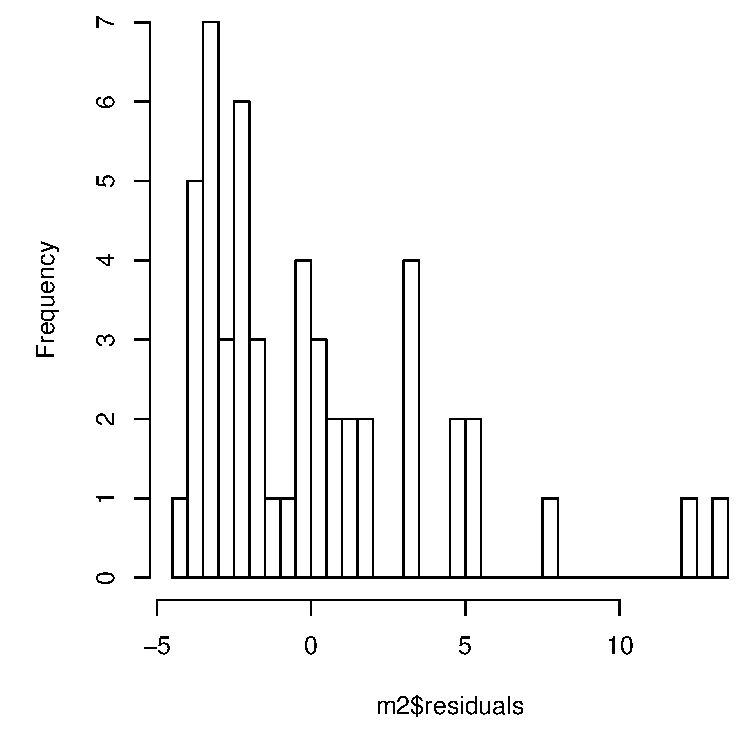
\includegraphics[width=0.8\linewidth]{figure/unnamed-chunk-4-2} 

\end{knitrout}

\end{columns}

\end{frame}
%===============================================================================%

%===============================================================================%
\begin{frame}{Distribuições dos parâmetros}

Contudo, geralmente queremos saber mais do que $\hat{Y}$:

\vfill
\begin{itemize}
  \item Qual o grau de certeza sobre $\hat Y$? \pause
  \item Qual o grau de certeza sobre $\beta _0$ e $\beta_1$? \pause
  \item Qual o grau de certeza sobre a relação entre $X$ e $Y$? \pause
  \item Com qual grau de certeza posso prever o valor esperado de $Y$? \pause
  \item Com qual grau de certeza posso prever um valor aleatório de $Y$? \pause
\end{itemize} 
\vfill
Para respondermos à essas perguntas, precisamos especificar uma distribuição de probabilidade para $\varepsilon$
\vfill
No modelo de regressão clássico, assumimos que esta distribuição é\ldots \pause
normal: $\varepsilon \sim N(0,\sigma ^2)$

\end{frame}
%===============================================================================%


%===============================================================================%
\begin{frame}{Pressuposições da regressão \ldots \emph{redux}}

\begin{equation*}
Y_i = \beta _0 + \beta _1 X_i + \varepsilon _i
\end{equation*} \pause

\begin{small}

\begin{enumerate}
  \item Existe uma relação linear entre $X$ e $Y$: $E(Y) = \beta _0 + \beta _1 X$. \pause
  \vfill
  \item Os erros $\varepsilon$ (e por consequência, $Y$) tem variância constante ($\sigma^2$). \pause
  \vfill
  \item Os erros $\varepsilon$ (e por consequência, $Y$) são independentes. \pause
  \vfill
  \item Os valores de $X$ são medidos sem erro (cada $X_i$ pode ser tratado como constante). \pause
  \vfill
  \item \alert{Os erros $\varepsilon$ (e por consequência, $Y$) são normalmente distribuídos:}
  \vfill
  \begin{itemize}
    \item \alert{$\varepsilon \sim N(0,\sigma^2)$}
    \vfill
    \item  \alert{$Y \sim N(\beta _0 + \beta _1 X,\sigma^2)$}
  \end{itemize}
\end{enumerate}

\end{small}
  
\end{frame}
%===============================================================================%

%===============================================================================%
\begin{frame}{Distribuição de probabilidade para $b_1$}

O parâmetro $b_1$ é um dos mais importantes em um modelo de regressão, porque\ldots \pause
nos diz qual o grau de relação entre $X$ e $Y$ (estima $\beta_1$). \pause
\vfill
Se $\beta_1 = 0$ ? \pause
\vfill
$E(Y) = \beta_0 + \varepsilon; \quad E(Y) \sim N(\beta_0, s^2); \quad E(Y) = \beta_0 = \bar{Y}$\pause

\vfill
$E(Y)$ é constante para qualquer nível de $X$, ou seja, não existe relação.

\end{frame}
%===============================================================================%

%===============================================================================%
\begin{frame}{Distribuição de probabilidade para $b_1$}

Analiticamente, nós havíamos determinado que:
\vfill
\begin{equation*}
b_1 = \frac{\sum(X_i - \bar X)(Y_i - \bar Y)}{\sum(X_i - \bar X)^2} \pause
\end{equation*}
\vfill
Podemos re-escrever essa equação como:
\vfill
\begin{equation*}
b_1 = \sum k_i Y_i; \thickspace  \thickspace \thickspace  k_i=\frac{(X_i - \bar X)}{\sum(X_i - \bar X)^2} \pause
\end{equation*}
\vfill
Ou seja, $b_1$ é uma combinação linear de valores de $Y_i$

\end{frame}
%===============================================================================%

%===============================================================================%
\begin{frame}{Distribuição de probabilidade para $b_1$}

\begin{columns}[c]

\column{0.7\linewidth}
\centering
\begin{small}

Então, se $Y_i \sim  N(\hat Y, s^2)$\ldots \pause

\end{small}

\bigskip
\centering
$b_1 \sim N \left( \beta _1,\frac{s^2}{\sum (X_i-\bar X)^2 \right)}$ \pause


\column{0.3\linewidth}


\includegraphics[width = 1\linewidth]{its_magic.jpg} \pause

\alert{ $\alert{\leftarrow}$
Isso também quer dizer que quanto maior a dispersão de $X$, mais certeza eu tenho sobre $b_1$}

\end{columns}

\end{frame}
%===============================================================================%


%===============================================================================%
\begin{frame}{Relembrando}


Quem é $s^2$? \pause
\vfill
\begin{itemize}
\item o nosso estimador de $\sigma^2$ \pause 
\vfill
\item A variância dos resíduos \pause
\end{itemize}

\begin{equation*}
SQ_{res} =\sum_{i-1}^{n}(Y_i - \hat Y)^2 = \sum_{i-1}^{n}e_i^2 \pause
\end{equation*}
\begin{equation*}
s^2 = MQ_{res} = \frac{SQ_{res}}{n-2} = \frac{\sum(Y_i - \hat Y)^2}{n-2} = \frac{\sum e_i^2}{n-2} \pause
\end{equation*}
\vfill
Então, calculamos a variância de $b_1$ como: 
\begin{equation*}
s^2_{b_1} = \frac{s^2}{\sum (X_i-\bar X)^2} = \frac{MQ_{res}}{\sum (X_i-\bar X)^2}
\end{equation*}

\end{frame}
%===============================================================================%


%===============================================================================%
\begin{frame}{Testando, testando, 1,2,3...}

\begin{small}

Se $X \sim N(\mu,\sigma^2)$, qual a distribuição de:
\vfill
\begin{equation*}
\frac{\bar X - \mu}{\sigma / \sqrt{n}} 
\end{equation*} \pause
\vfill
$\mu=$ média populacional; 

$\bar X =$ estimador de $\mu$; 

$\sigma / \sqrt{n} =$ erro padrão da média populacional (estima $\sqrt{Var(\mu)}$)\pause

\begin{equation*}
\frac{\bar X - \mu}{\sigma / \sqrt{n}} = Z \pause
\end{equation*}
\vfill
\begin{equation*}
Z \sim N(0,1) 
\end{equation*}

\end{small}

\end{frame}
%===============================================================================%

%===============================================================================%
\begin{frame}{Testando, testando, 1,2,3...}

Mas nós não conhecemos $\sigma$, só conhecemos $s$ (amostra).$
\vfill
\begin{equation*}
\frac{\bar X - \mu}{s / \sqrt{n}} 
\end{equation*} \pause
\vfill
$\mu=$ média populacional; 

$\bar X =$ estimador de $\mu$; 

$s / \sqrt{n} =$ erro padrão da média amostral (estima $\sqrt{Var(\bar X)}$)
\vfill
Qual a distribuição desta nova variável?\pause

\begin{equation*}
\frac{\bar Y - \mu}{s / \sqrt{n}} = T \pause
\end{equation*}
\vfill
\begin{equation*}
t \sim t({n-1}) 
\end{equation*}


\end{frame}
%===============================================================================%


% %===============================================================================%
% \begin{frame}{A distribuição $t$ de Student}
% 
% \begin{itemize}
%   \item Student = William Gosset
%   \vfill
%   \item Pelo Teorema do Limite Central, $s$ aproxima $\sigma$ para "grandes" amostras ($n \geq 30$). Mas, se as amostras são pequenas, isso não vale.
%   \item Para pequenas amostras, essa estatística se aproxima mais de uma distribuição $t$
%   \item O único parâmetro de $t$ é $(n-v)$, ou seja, os graus de liberdade.
%   \item Quando ($n \geq 30$), $t$ se aproxima de uma distribuição normal.
% \end{itemize}
% 
% \end{frame}
% %===============================================================================%
% 
% 
% %===============================================================================%
% \begin{frame}[fragile]
% 
% <<echo=F, fig.height = 5, fig.width = 5, out.width = "0.8\\linewidth">>=
% x <- seq(-4, 4, length=100)
% hx <- dnorm(x)
% 
% degf <- c(1, 3, 8, 30)
% colors <- c("red", "blue", "darkgreen", "gold", "black")
% labels <- c("df=1", "df=3", "df=8", "df=30", "normal")
% 
% plot(x, hx, type="l", lty=2, xlab=NA,
%   ylab="Density", main="Comparison of t Distributions")
% 
% for (i in 1:4){
%   lines(x, dt(x,degf[i]), lwd=2, col=colors[i])
% }
% 
% legend("topright", inset=.05, title="Distributions",
%   labels, lwd=2, lty=c(1, 1, 1, 1, 2), col=colors)
% @
% 
% 
% 
% \end{frame}
% %===============================================================================%
% 
% 
% 

%===============================================================================%
\begin{frame}{I.C. e Teste de Hipóteses para $\beta _1$}

\begin{columns}[c]

\column{0.7\linewidth}
\begin{small}
E se \ldots usarmos $b_1$ e $\beta _1$ em vez de $\bar X$ e $\mu$? \pause
\vfill
\begin{equation*}
\frac{b_1 - \beta _1}{\alert{?}} = t
\end{equation*} \pause
\vfill
$s / \sqrt{n}$ era o estimador de $\sqrt{Var(\bar X)}$
Quem é o nosso estimador de $\sqrt{s^2_{b_1}}$? \pause 
\begin{equation*}
\frac{b_1 - \beta _1}{\sqrt{s^2_{b_1}}} =  \frac{b_1 - \beta _1}{\sqrt{\frac{MQ_{res}}{\sum (X_i-\bar X)^2}}} = t \sim t_{n-2}
\end{equation*} \pause
\vfill
\textbf{Agora podemos fazer inferências sobre $\beta _1$!}
\end{small}
\column{0.3\linewidth}


\includegraphics[width = 1\linewidth]{heman.png}

\end{columns}

\end{frame}
%===============================================================================%


%===============================================================================%
\begin{frame}{Intervalos de Confiança}

\begin{small}

\textbf{Intervalos de confiança }são uma maneira diferente de expressar o seu grau de certeza sobre as suas estimativas. A sua construção é paramétrica e segue o mesmo procedimento do valor $p$.
\vfill
\alert{\textbf{Exemplo:}} Coletei 20 observações de uma amostra, a qual teve média $\bar{X} = 10$ e desvio padrão $s = 5$. Qual o intervalo de confiança para essa média? \pause


Poderíamos assumir uma distribuição Normal: $\bar{X} \sim N(\bar{X},s/\sqrt{n})$. A partir daí, só precisaríamos calcular os valores correspondentes a $\alpha = 0.05$, bi-caudal.

\end{small}

\end{frame}
%===============================================================================%


%===============================================================================%
\begin{frame}[fragile]{Intervalos de Confiança}

\begin{knitrout}\tiny
\definecolor{shadecolor}{rgb}{0.969, 0.969, 0.969}\color{fgcolor}\begin{kframe}
\begin{alltt}
\hlcom{# Se o teste é bi-caudal, dividimos a probabilidade de 0.05}
\hlcom{# entre as duas caudas da distribuição}

\hlstd{x_bar} \hlkwb{<-} \hlnum{10}
\hlstd{s} \hlkwb{<-} \hlnum{5}
\hlstd{n} \hlkwb{<-} \hlnum{20}

\hlkwd{qnorm}\hlstd{(}\hlnum{0.025}\hlstd{,}\hlkwc{mean}\hlstd{=x_bar,}\hlkwc{sd}\hlstd{=s}\hlopt{/}\hlkwd{sqrt}\hlstd{(n))}
\end{alltt}
\begin{verbatim}
## [1] 7.808694
\end{verbatim}
\begin{alltt}
\hlkwd{qnorm}\hlstd{(}\hlnum{0.975}\hlstd{,}\hlkwc{mean}\hlstd{=x_bar,}\hlkwc{sd}\hlstd{=s}\hlopt{/}\hlkwd{sqrt}\hlstd{(n))}
\end{alltt}
\begin{verbatim}
## [1] 12.19131
\end{verbatim}
\end{kframe}
\end{knitrout}

\begin{small}


Nosso I.C. para $\bar{X}$ é $P(7.8 \leq \bar{X} \leq 12.2) = 0.95$.

Ou seja, se repetíssemos a mesma amostragem infinitamente, a média estaria entre esses valores 95\% das vezes. 

\end{small}

\end{frame}
%===============================================================================%


%===============================================================================%
\begin{frame}[fragile]{Intervalos de Confiança}

\begin{small}

Poderíamos também assumir uma distribuição t: 

$\frac{\bar{X}}{s/\sqrt{n}} ~ \sim t(\nu = n-1)$. 

Nesse caso, primeiro calculamos os valores de $t$ que correspondem a $\alpha= 0.05$, e depois multiplicamos esse valor por $s/\sqrt{n}$ 

\end{small}

\vfill

\begin{knitrout}\tiny
\definecolor{shadecolor}{rgb}{0.969, 0.969, 0.969}\color{fgcolor}\begin{kframe}
\begin{alltt}
\hlstd{se} \hlkwb{<-} \hlstd{s}\hlopt{/}\hlkwd{sqrt}\hlstd{(n)}

\hlstd{x_bar} \hlopt{+} \hlkwd{qt}\hlstd{(}\hlnum{0.025}\hlstd{,n}\hlopt{-}\hlnum{1}\hlstd{)}\hlopt{*} \hlstd{se}
\end{alltt}
\begin{verbatim}
## [1] 7.659928
\end{verbatim}
\begin{alltt}
\hlstd{x_bar} \hlopt{+} \hlkwd{qt}\hlstd{(}\hlnum{0.975}\hlstd{,n}\hlopt{-}\hlnum{1}\hlstd{)}\hlopt{*} \hlstd{se}
\end{alltt}
\begin{verbatim}
## [1] 12.34007
\end{verbatim}
\end{kframe}
\end{knitrout}

\end{frame}
%===============================================================================%


%===============================================================================%
\begin{frame}{I.C. e Teste de Hipóteses para $\beta _1$}

O intervalo de confiança para $\beta _1$ é:
\begin{equation*}
P(b_1 - t^* \times s_{b_1} \leq \beta _1 \leq b_1 + t^* \times s_{b_1} ) =  1 - \alpha
\end{equation*} \pause
Onde $t^* = t(1-\alpha/2;n-2)$ \pause
\vfill
E podemos testar a hipótese $H_0: \beta _1 = 0$ usando
\begin{equation*}
t^* = \frac{b_1 - \beta _1}{s_{b_1}} = \frac{b_1 - 0}{s_{b_1}} = \frac{b_1}{s_{b_1}}
\end{equation*}

Quanto menor o valor de $p$, mais temos certeza sobre o valor estimado de $\beta_1$


\end{frame}
%===============================================================================%


%===============================================================================%
\begin{frame}{Distribuição de probabilidade para $b_0$}

Assim, como $b_1$, $b_0$ é uma combinação linear de valores de $Y_i$ (acreditem)

\begin{equation*}
b_0 = \bar Y - b_1 \bat X \pause
\end{equation*}

Por esse motivo, a distribuição de $b_0$ também é normal, com:

\begin{equation*}
E(b_0) = \beta _0 \pause
\end{equation*}

\begin{equation*}
s^2_{b_0} = MQ_{res} \left( \frac{1}{n} + \frac{{\bar X}^2}{\sum (X_i - \bar X)^2 \right)}
\end{equation*}

\end{frame}
%===============================================================================%


%===============================================================================%
\begin{frame}{I.C. e Teste de Hipóteses para $\beta _0$}

A construção de um I.C. para $\beta _0$ é:
\begin{equation*}
P(b_0 - t^* \times s_{b_0} \leq \beta _0 \leq b_0 + t^* \times s_{b_0} ) =  1 - \alpha
c\end{equation*}
Onde $t^* = t(1-\alpha/2;n-2)$ \pause
\vfill
E podemos testar a hipótese $H_0: \beta _0 = 0$ usando
\begin{equation*}
t^* = \frac{b_0 - \beta _0}{s_{b_0}} = \frac{b_0 - 0}{s_{b_0}} = \frac{b_0}{s_{b_0}}
\end{equation*}

Quanto menor o valor de $p$, mais temos certeza sobre o valor estimado de $\beta_1$

\end{frame}
%===============================================================================%


%===============================================================================%
\begin{frame}{Distribuição de probabilidade para $\hat{Y}_h$}

Adivinhem: $\hat Y_h$ ($h$ significando um nível qualquer de X) é\ldots \pause uma combinação linear dos valores de $Y_i$
\vfill
Por esse motivo, a distribuição de $\hat Y_h$ também é normal, com:

\begin{equation*}
E(\hat Y_h) = E(Y_h) 
\end{equation*}

\only<3>{
\begin{equation*}
s^2_{\hat Y_h} = MQ_{res} \left( \frac{1}{n} + \frac{(X_h - \bar X)^2}{\sum (X_i - \bar X)^2 \right)}
\end{equation*}
}

\only<4>{
\begin{equation*}
s^2_{\hat{Y}_h} = MQ_{res} \left( \frac{1}{n} + \frac{\alert{(X_h - \bar X)^2}}{\sum (X_i - \bar X)^2 \right)}
\end{equation*}

\begin{alertblock}{Atenção!}
{Quanto mais longe estivermos de $\bar{X}$ ao longo da reta, maior a incerteza sobre $\hat{Y}$!}
\end{alertblock}
}

\end{frame}
%===============================================================================%


%===============================================================================%
\begin{frame}{I.C. e Teste de Hipóteses para $E(Y_h)$}

A construção de um I.C. para $E(Y_h)$ é:
\begin{equation*}
P(\hat Y_h - t^* \times s_{\hat Y_h} \leq E(Y_h) \leq \hat Y_h + t^* \times s_{\hat Y_h} ) =  1 - \alpha
\end{equation*}
Onde $t^* = t(1-\alpha/2;n-2)$ \pause
\vfill
Dificilmente fará sentido testar se $E(Y_h) = 0$, mas podemos testar a hipótese $H_0: E(Y_h) = H$  para um valor $H$ qualquer, usando
\begin{equation*}
t^* = \frac{\hat Y_h - H}{s_{\hat Y_h}} 
\end{equation*}

\end{frame}
%===============================================================================%


%===============================================================================%
\begin{frame}{Predição de um novo valor:$Y_{h(novo)}$}

Um dos principais usos de um modelo de regressão é a predição de novos valores de $Y$, dado um certo $X_h$. Chamaremos esse novo valor de $Y_{h(novo)}$. \pause
\vfill
Mas já sabemos calcular o I.C. para $E(Y_h)$\ldots não é a mesma coisa? \pause
\vfill
No caso de $E(Y_h)$, estamos considerando a distribuição da esperança (média). Quando falamos de $Y_{h(novo)}$, estamos considerando a  distribuição \textbf{de todos os valores possíveis} de $Y$ para $X = X_h$.

\end{frame}
%===============================================================================%


%===============================================================================%
\begin{frame}[fragile]{Diferença entre I.C. de $E(Y_h)$ e I.C. de $Y_{h(novo)}$}
\centering
\begin{knitrout}
\definecolor{shadecolor}{rgb}{0.969, 0.969, 0.969}\color{fgcolor}
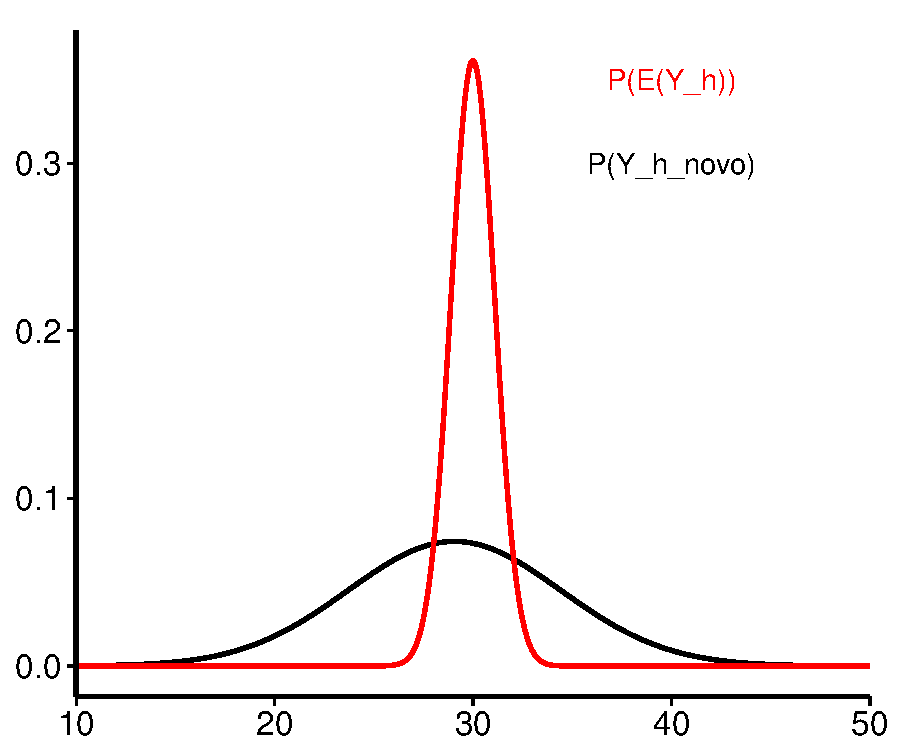
\includegraphics[width=0.8\linewidth]{figure/unnamed-chunk-7-1} 

\end{knitrout}


\end{frame}
%===============================================================================%

%===============================================================================%
\begin{frame}{Diferença entre I.C. de $E(Y_h)$ e I.C. de $Y_{h(novo)}$}
\centering
\begin{knitrout}
\definecolor{shadecolor}{rgb}{0.969, 0.969, 0.969}\color{fgcolor}
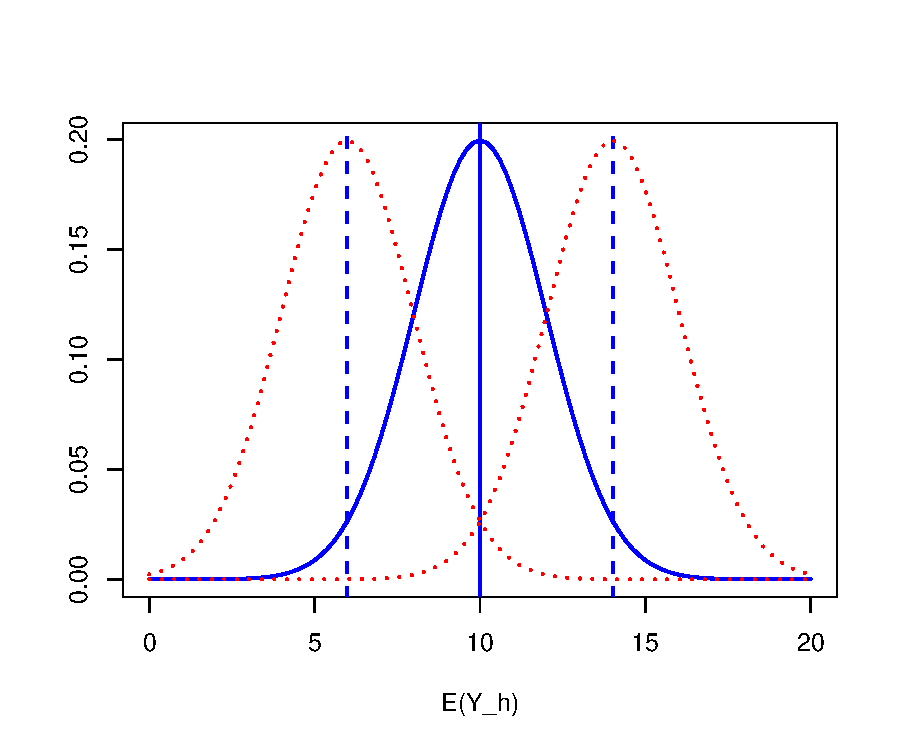
\includegraphics[width=0.8\linewidth]{figure/unnamed-chunk-8-1} 

\end{knitrout}

\end{frame}
%===============================================================================%

%===============================================================================%
\begin{frame}{I.C. para $Y_{h(novo)}$}

Utilizando novamente a distribuição $t$ de Student, podemos usar:

\begin{equation*}
t = \frac{Y_{h(novo)}- \hat Y_h}{s_{Y_{h(novo)}}}
\end{equation*}

E através das mágicas propriedades da esperança e variância, podemos dizer que:

\begin{equation*}
\sigma^2_{Y_{h(novo)}} = \sigma ^2 + \sigma^2 _{\hat Y_h}
\end{equation*}

\begin{equation*}
s^2_{Y_{h(novo)}} = MQ_{res} \left( 1 + \frac{1}{n} + \frac{(X_h - \bar X)^2}{\sum(X_i - \bar X)^2} \right)
\end{equation*}

\end{frame}
%===============================================================================%


%===============================================================================%
\begin{frame}
\centering

\includegraphics[width = 1\linewidth]{The_Scream.jpg}

\end{frame}
%===============================================================================%


%===============================================================================%
\begin{frame}{Exemplo}

\begin{scriptsize}
Decidimos investigar a relação entre duas variáveis. Primeiro fazemos uma inspeção dos dados:

\end{scriptsize}

\begin{columns}[c]

\column{0.5\linewidth}
\begin{knitrout}
\definecolor{shadecolor}{rgb}{0.969, 0.969, 0.969}\color{fgcolor}
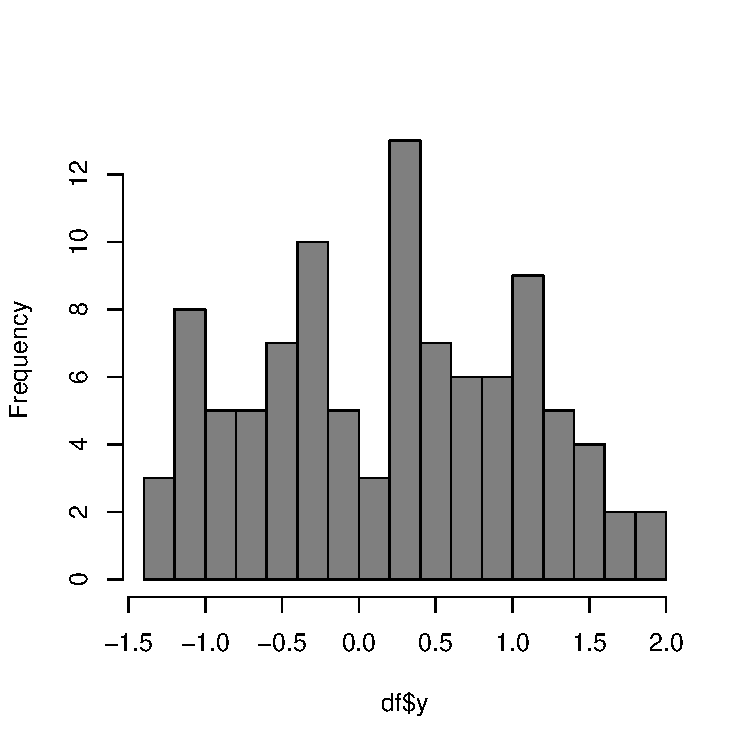
\includegraphics[width=1\linewidth]{figure/histoiaf-1} 

\end{knitrout}


\column{0.5\linewidth}
\begin{knitrout}
\definecolor{shadecolor}{rgb}{0.969, 0.969, 0.969}\color{fgcolor}
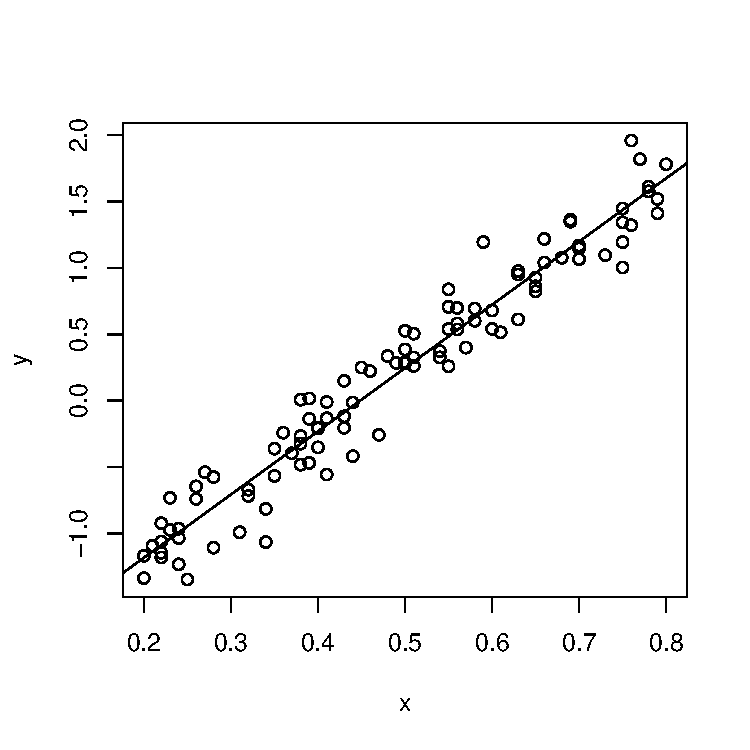
\includegraphics[width=1\linewidth]{figure/scatteriaf-1} 

\end{knitrout}

\end{columns}
\end{frame}
%===============================================================================%


%===============================================================================%
\begin{frame}[fragile]{Exemplo}

\begin{scriptsize}
Os dados aparentam ter uma relação linear, e a variável dependente parece ser normalmente distribuída, então podemos ajustar um modelo de regressão: \pause
\end{scriptsize}

\bigskip

\begin{columns}[c]

\column{0.5\linewidth}

\begin{knitrout}\tiny
\definecolor{shadecolor}{rgb}{0.969, 0.969, 0.969}\color{fgcolor}\begin{kframe}
\begin{alltt}
\hlstd{m1} \hlkwb{<-} \hlkwd{lm}\hlstd{(y} \hlopt{~} \hlstd{x,}\hlkwc{data}\hlstd{=df)}
\hlstd{m1}\hlopt{$}\hlstd{coefficients}
\end{alltt}
\begin{verbatim}
## (Intercept)           x 
##   -2.134360    4.760905
\end{verbatim}
\begin{alltt}
\hlkwd{anova}\hlstd{(m1)[}\hlnum{1}\hlopt{:}\hlnum{3}\hlstd{]}
\end{alltt}
\begin{verbatim}
##           Df Sum Sq Mean Sq
## x          1 69.185  69.185
## Residuals 98  4.040   0.041
\end{verbatim}
\begin{alltt}
\hlkwd{var}\hlstd{(df}\hlopt{$}\hlstd{y)}\hlopt{*}\hlnum{99}
\end{alltt}
\begin{verbatim}
## [1] 73.22441
\end{verbatim}
\end{kframe}
\end{knitrout}

\column{0.5\linewidth}

$\bar{Y_i} = -2.13 + 4.76 \times X$ \pause
\vfill
$\sum(e_i)^2 =SQ_{res} = 4$ \pause
\vfill
$\sum(Y_i -\bar Y)^2 = SQ_{tot} = 73.2$ \pause
\vfill
$SQ_{reg} = SQ_{tot} - SQ_{res} =  69.2$ \pause
\vfill
$\sum (X_i - \bar X)^2 = 3.05$ 
\vfill
$\bar X = 0.489$
\end{columns}
\end{frame}
%===============================================================================%


%===============================================================================%
\begin{frame}[fragile]{Exemplo}

1) Qual o $r^2$ desse modelo? \pause

\begin{equation*}
r^2 = \frac{SQ_{reg}}{SQ_{tot}} = \frac{69.2}{73.2} = 0.945 \pause
\end{equation*}

\begin{knitrout}\tiny
\definecolor{shadecolor}{rgb}{0.969, 0.969, 0.969}\color{fgcolor}\begin{kframe}
\begin{alltt}
\hlkwd{summary}\hlstd{(miaf)}\hlopt{$}\hlstd{r.squared}
\end{alltt}
\begin{verbatim}
## [1] 0.9448324
\end{verbatim}
\end{kframe}
\end{knitrout}


\end{frame}
%===============================================================================%

%===============================================================================%
\begin{frame}{Exemplo}

2) Qual o I.C. para $\beta _1$, quando $\alpha=0.5$? \pause
\vfill
$\frac{b_1 - \beta _1}{s_{b_{1}}} \sim t(n-2); \quad H_0: \beta_1 = 0; \quad t^{*}_{(\alpha/2,n-2)} =  ?$ \pause
\vfill
$s_{b_1} = \sqrt{\frac{MQ_{res}}{\sum (X_i-\bar X)^2}} = \sqrt{\frac{\frac{SQ_{res}}{(n-2)}}{\sum (X_i-\bar X)^2}} = \sqrt{\frac{\frac{4}{98}}{3.05}} =  \sqrt{0.013} = 0.116$ \pause
\vfill
$P(b_1 - t^* \times s_{b_1} \leq \beta _1 \leq b_1 + t^* \times s_{b_1} ) =  1 - \alpha$ \pause
\vfill
$P(4.76 - 1.98 \times 0.116 \leq \beta _1 \leq 4.76 + 1.98 \times 0.116 ) =  0.95$ \pause
\vfill
$P(4.53 \leq \beta _1 \leq 4.99) = 0.95$

\end{frame}
%===============================================================================%

%===============================================================================%
\begin{frame}[fragile]{Exemplo}

\begin{knitrout}\tiny
\definecolor{shadecolor}{rgb}{0.969, 0.969, 0.969}\color{fgcolor}\begin{kframe}
\begin{alltt}
 \hlkwd{summary}\hlstd{(m1)}\hlopt{$}\hlstd{coefficients}
\end{alltt}
\begin{verbatim}
##              Estimate Std. Error   t value     Pr(>|t|)
## (Intercept) -2.134360 0.06031152 -35.38893 1.256108e-57
## x            4.760905 0.11620932  40.96836 1.818830e-63
\end{verbatim}
\begin{alltt}
\hlnum{4.76} \hlopt{-} \hlnum{1.98}\hlopt{*}\hlnum{0.11621}
\end{alltt}
\begin{verbatim}
## [1] 4.529904
\end{verbatim}
\begin{alltt}
\hlnum{4.76} \hlopt{+} \hlnum{1.98}\hlopt{*}\hlnum{0.11621}
\end{alltt}
\begin{verbatim}
## [1] 4.990096
\end{verbatim}
\begin{alltt}
\hlkwd{confint}\hlstd{(m1)}
\end{alltt}
\begin{verbatim}
##                 2.5 %    97.5 %
## (Intercept) -2.254047 -2.014674
## x            4.530292  4.991519
\end{verbatim}
\end{kframe}
\end{knitrout}


\end{frame}
%===============================================================================%


%===============================================================================%
\begin{frame}{Exemplo}

3) Qual o I.C. para $\beta _0$, quando $\alpha=0.5$? \pause
\vfill
$\frac{b_0 - \beta _0}{s_{b_{0}}} \sim t(n-2); \quad H_0: \beta_0 = 0; \quad t^{*}_{(\alpha/2,n-2)} =  ?$ \pause
\vfill
$s_{b_0} = \sqrt{MQ_{res} \left( \frac{1}{n} + \frac{{\bar X}^2}{\sum (X_i - \bar X)^2 \right)}} = \sqrt{\frac{4}{98} \left( \frac{1}{100} + \frac{0.24}{3.05 \right)}} = 0.06$ \pause
\vfill
$P(b_0 - t^* \times s_{b_0} \leq \beta _0 \leq b_0 + t^* \times s_{b_0} ) =  1 - \alpha$ \pause
\vfill
$P(-2.13 - 1.98 \times 0.06 \leq \beta _1 \leq -2.13 + 1.98 \times 0.06 ) =  0.95$ \pause
\vfill
$P(-2.25 \leq \beta _0 \leq -2.01) = 0.95$

\end{frame}
%===============================================================================%

%===============================================================================%
\begin{frame}[fragile]{Exemplo}

\begin{knitrout}\tiny
\definecolor{shadecolor}{rgb}{0.969, 0.969, 0.969}\color{fgcolor}\begin{kframe}
\begin{alltt}
 \hlkwd{summary}\hlstd{(miaf)}\hlopt{$}\hlstd{coefficients}
\end{alltt}
\begin{verbatim}
##              Estimate Std. Error   t value     Pr(>|t|)
## (Intercept) -2.134360 0.06031152 -35.38893 1.256108e-57
## x            4.760905 0.11620932  40.96836 1.818830e-63
\end{verbatim}
\begin{alltt}
\hlopt{-}\hlnum{2.13} \hlopt{-} \hlnum{1.98}\hlopt{*}\hlnum{0.06031}
\end{alltt}
\begin{verbatim}
## [1] -2.249414
\end{verbatim}
\begin{alltt}
\hlopt{-}\hlnum{2.13} \hlopt{+} \hlnum{1.98}\hlopt{*}\hlnum{0.06031}
\end{alltt}
\begin{verbatim}
## [1] -2.010586
\end{verbatim}
\begin{alltt}
\hlkwd{confint}\hlstd{(m1)}
\end{alltt}
\begin{verbatim}
##                 2.5 %    97.5 %
## (Intercept) -2.254047 -2.014674
## x            4.530292  4.991519
\end{verbatim}
\end{kframe}
\end{knitrout}


\end{frame}
%===============================================================================%

%===============================================================================%
\begin{frame}{Exemplo}

4) Qual o valor esperado de $\hat{Y}_h$ e seu I.C. quando $X_h=0.5$ ? \pause
\vfill

$\frac{\hat{Y}_h - E(Y_h)}{s_{\hat{Y}_{h}}} \sim t(n-2); \quad H_0: E(Y_h) = 0; \quad t^{*}_{(\alpha/2,n-2)} =  ?$ \pause
\vfill
$s_{\hat{Y}_h} = \sqrt{MQ_{res} \left( \frac{1}{n} + \frac{(X_h - \bar X)^2}{\sum (X_i - \bar X)^2} \right)}  = \sqrt{\frac{4}{98} \left( \frac{1}{100} + \frac{(0.5 - 0.489)^2}{3.05} )\right} = 0.02 $ \pause
\vfill
$P(\hat Y_h - t^* \times s_{\hat Y_h} \leq \hat E(Y_h) \leq \hat Y_h + t^* \times s_{\hat Y_h} ) =  1 - \alpha$ \pause
\vfill
$P(0.25 - 1.98 \times 0.02 \leq E(Y_h) \leq 0.25 + 1.98 \times 0.02 ) =  0.95$ \pause
\vfill
$P(0.21 \leq E(Y_h) \leq 0.28) = 0.95$

\end{frame}
%===============================================================================%


%===============================================================================%
\begin{frame}{Exemplo}

5) Qual o intervalo de predição de $\hat{Y}_{h(novo)}$ quando $X_h=0.5$ ? \pause

s_{\hat Y_{h(novo)}} = \sqrt{MQ_{res} \left( 1 + \frac{1}{n} + \frac{(X_h - \bar X)^2}{\sum(X_i - \bar X)^2} \right)}  = \sqrt{\frac{4}{98} \left(1 + \frac{1}{100} + \frac{(0.5 - 0.489)^2}{3.05} )\right} = 0.203 $ \pause
\vfill
$P(\hat Y_{h} - t^* \times s_{\hat Y_{h(novo)}} \leq Y_{h(novo)} \leq \hat Y_{h} + t^* \times s_{\hat Y_{h(novo)}} ) =  1 - \alpha$ \pause
\vfill
$P(0.25 - 1.98 \times 0.203 \leq Y_{h(novo)} \leq 0.25 + 1.98 \times 0.203 ) =  0.95$ \pause
\vfill
$P(-0.152 \leq Y_{h(novo)} \leq 0.652) = 0.95$

\end{frame}
%===============================================================================%
 
 
 %===============================================================================%
\begin{frame}[fragile]

$P(0.21 \leq E(Y_h) \leq 0.28) = 0.95$
\vfill
$P(-0.152 \leq Y_{h(novo)} \leq 0.652) = 0.95$
\vfill
\begin{knitrout}\tiny
\definecolor{shadecolor}{rgb}{0.969, 0.969, 0.969}\color{fgcolor}\begin{kframe}
\begin{alltt}
\hlkwd{predict}\hlstd{(m1,newobs,}\hlkwc{interval}\hlstd{=}\hlstr{'confidence'}\hlstd{)}
\end{alltt}
\begin{verbatim}
##         fit       lwr       upr
## 1 0.2460923 0.2057178 0.2864668
\end{verbatim}
\begin{alltt}
\hlkwd{predict}\hlstd{(m1,newobs,}\hlkwc{interval}\hlstd{=}\hlstr{'prediction'}\hlstd{)}
\end{alltt}
\begin{verbatim}
##         fit        lwr       upr
## 1 0.2460923 -0.1588289 0.6510134
\end{verbatim}
\end{kframe}
\end{knitrout}

\end{frame}
%===============================================================================%
 
 
%===============================================================================%
\begin{frame}[fragile]

\begin{knitrout}\tiny
\definecolor{shadecolor}{rgb}{0.969, 0.969, 0.969}\color{fgcolor}\begin{kframe}
\begin{alltt}
\hlkwd{summary}\hlstd{(m1)}
\end{alltt}
\begin{verbatim}
## 
## Call:
## lm(formula = y ~ x, data = df)
## 
## Residuals:
##      Min       1Q   Median       3Q      Max 
## -0.54883 -0.11846  0.01314  0.14513  0.51984 
## 
## Coefficients:
##             Estimate Std. Error t value Pr(>|t|)    
## (Intercept) -2.13436    0.06031  -35.39   <2e-16 ***
## x            4.76091    0.11621   40.97   <2e-16 ***
## ---
## Signif. codes:  0 '***' 0.001 '**' 0.01 '*' 0.05 '.' 0.1 ' ' 1
## 
## Residual standard error: 0.203 on 98 degrees of freedom
## Multiple R-squared:  0.9448,	Adjusted R-squared:  0.9443 
## F-statistic:  1678 on 1 and 98 DF,  p-value: < 2.2e-16
\end{verbatim}
\end{kframe}
\end{knitrout}

\end{frame}
%===============================================================================%


%===============================================================================%
\begin{frame}{Ok, pra que serve tudo isso?}

\begin{itemize}
 \item Inferências sobre $\beta _1$ nos dizem a certeza acerca da relação entre $X$ e $Y$  \pause
\vfill
\item Inferências sobre $\beta _0$ nos dizem se a reta passa pela origem ($\beta _0 = 0$) \pause
\vfill
\item Inferências sobre $E(Y_h)$ nos dizem a certeza acerca do valor esperado de $Y_i$ para um dado $X_i$ ($E[Y_i]$) \pause
\vfill
\item Inferências sobre $Y_{h(novo)}$ nos dizem a certeza acerca de um valor aleatório de $Y_i$, para um dado $X_i$ \pause
\vfill
\item Só isso!
\end{itemize}
\end{frame}
%===============================================================================%

\section{Relembrando: partição de variância}


%===============================================================================%
\begin{frame}{Relembrando: partição de variância}

Um dos objetivos de um modelo de regressão linear é quantificar o quanto da variação total em $Y$ nós podemos explicar através de $X$
\vfill
Para isso, usamos o método de partição de variâncias: $SQ_{tot}$, $SQ_{res}$ e $SQ_{reg}$
\vfill
\begin{itemize}
  \item Soma dos Quadrados Totais? \pause $\sum(Y_i-\bar Y)^2$ \pause
  \vfill
  \item Soma dos Quadrados dos Erros? \pause $\sum(Y_i-\hat Y_i)^2$ \pause
  \vfill
  \item Soma dos Quadrados da Regressão? \pause $\sum(\hat Y_i - \bar Y)^2$
\end{itemize}

\end{frame}
%===============================================================================%


%===============================================================================%
\begin{frame}{Relembrando: partição de variância}



\begin{columns}[c]

\column{0.33\linewidth}

\begin{knitrout}
\definecolor{shadecolor}{rgb}{0.969, 0.969, 0.969}\color{fgcolor}
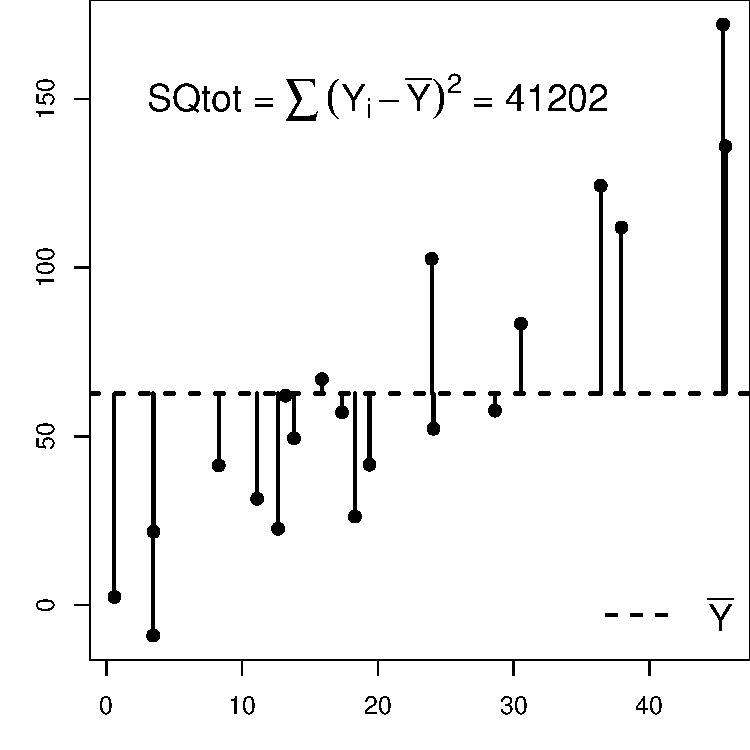
\includegraphics[width=1.1\linewidth]{figure/plotsqt-1} 

\end{knitrout}

\pause

\column{0.33\linewidth}

\begin{knitrout}
\definecolor{shadecolor}{rgb}{0.969, 0.969, 0.969}\color{fgcolor}
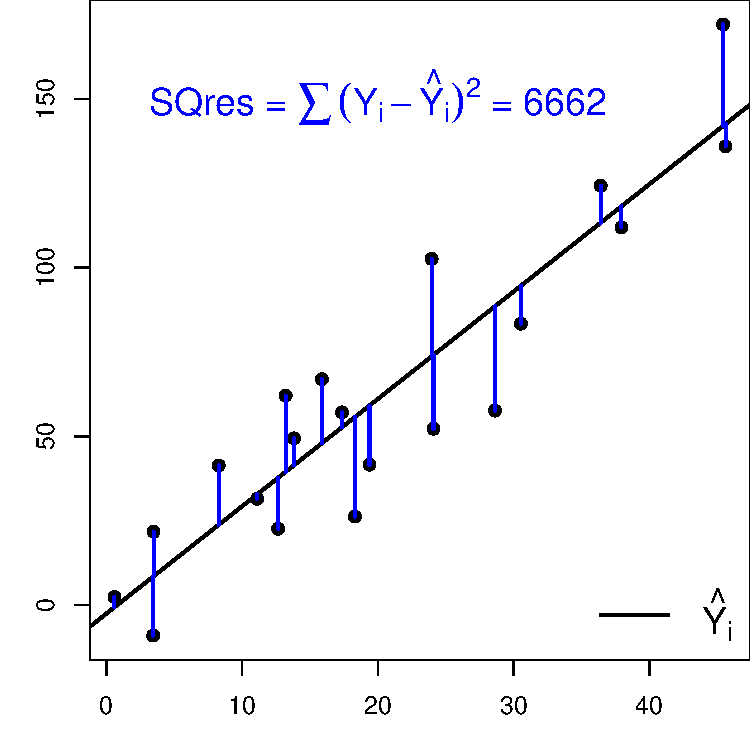
\includegraphics[width=1.1\linewidth]{figure/plotsqE-1} 

\end{knitrout}

\pause

\column{0.33\linewidth}

\begin{knitrout}
\definecolor{shadecolor}{rgb}{0.969, 0.969, 0.969}\color{fgcolor}
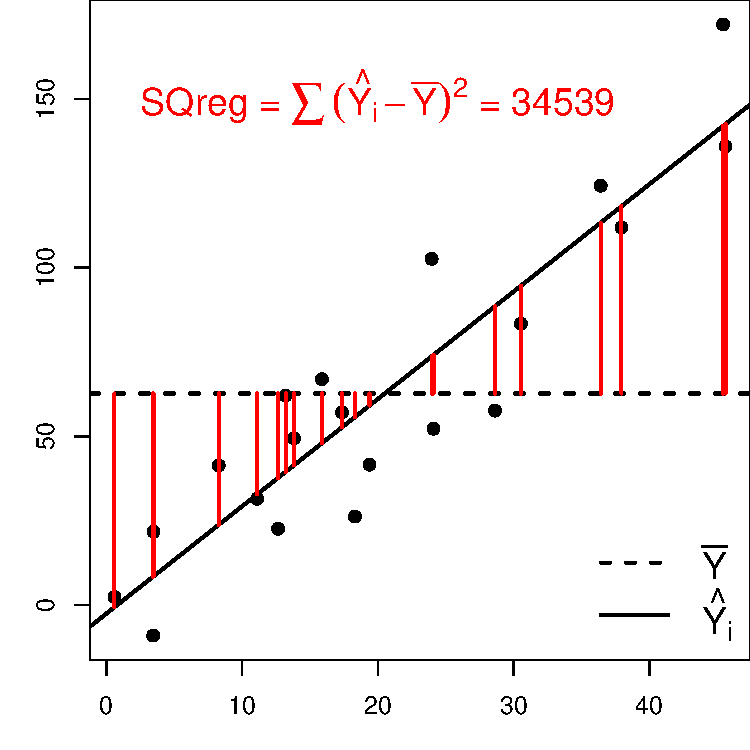
\includegraphics[width=1.1\linewidth]{figure/plotsqr-1} 

\end{knitrout}

\end{columns}

\end{frame}
%===============================================================================%

\section{Tabela ANOVA e teste F para regressão}


%===============================================================================%
\begin{frame}{A tabela ANOVA para regressão}

Uma maneira comum para mostrar a partição dos erros em um modelo de regressão é a \textbf{tabela ANOVA} \pause
\vfill
ANOVA significa \emph{ANalysis Of VAriance} (Análise de Variância) \pause
\vfill
A ANOVA pode ser vista como uma "versão" da regressão, um método para particionar as variâncias quando $X$ é categórico \pause
\vfill
De fato, ANOVA e Regressão Linear são casos específicos dos chamados Modelos Lineares Gerais (e um teste $t$ é uma ANOVA com apenas dois tratamentos).

\end{frame}
%===============================================================================%


%===============================================================================%
\begin{frame}{A tabela ANOVA para regressão}

Elementos de uma tabela ANOVA completa
\vfill

\resizebox{\textwidth}{!}{%
\begin{tabular}{lcllccc}
Fonte & GL & Soma Quadrados & Média Quadrados & E(Med. Quad.) & F & P \\
\hline
& & & & & &\\
Regressão & 1 & $SQ_{reg} = \sum(\hat Y_i - \bar Y)^2$ & $MQR = \dfrac{SQ_{reg}}{1}$ & \alert{$\sigma^2+\beta _1 ^2 \sum{(X_i - \bar X)^2}}$ & $\dfrac{MQR}{MQE} & P(F_{(1,n-2)}) \\[5ex]
Resíduos & $n-2$ & $SQ_{res} = \sum(Y_i - \hat Y_i)^2$ & $MQE = \dfrac{SQ_{res}}{n-2}$ & $\sigma^2$ & &  \\[5ex]
Total & $n-1$ & $SQ_{tot} = \sum(Y_i - \bar Y)^2$ & $MQT = \dfrac{SQ_{tot}}{n-1}$ & $\sigma^2 _Y$ & &  \\[5ex]
\hline
\end{tabular}%
}

\end{frame}
%===============================================================================%


%===============================================================================%
\begin{frame}{Distribuindo...}

Se $X \sim N(\mu,\sigma^2)$, qual a distribuição de:
\vfill
\begin{equation*}
\frac{\sum(X_i - \mu)^2}{\sigma^2} = \pause \chi ^2 _n
\end{equation*} \pause
\vfill
E qual a distribuição de: 
\begin{equation*}
\frac{\sum(X_i - \bar X)^2}{s^2} = \pause \chi ^2 _{n-1}
\end{equation*} 

\end{frame}
%===============================================================================%


%===============================================================================%
\begin{frame}{Distribuindo}

E se $U_1 \sim \chi ^2 _{gl_1}$ e $U_2 \sim \chi ^2 _{gl_1}$, qual a distribuição de:
\vfill
\begin{equation*}
\frac{U_1/gl_1}{U_2/gl_2} = \pause F _{gl_1,gl_2}
\end{equation*}

\end{frame}
%===============================================================================%


%===============================================================================%
\begin{frame}{Hmmmmm....}


$U = \dfrac{\sum(X_i - \bar X)^2}{s^2} \sim \chi ^2 _{n-1} \mspace{15mu} ; \mspace{15mu} \dfrac{U_1/gl_1}{U_2/gl_2} \sim F _{gl_1,gl_2}$  \pause
\vfill
Se a variância é constante, então: \pause
\vfill
$  \dfrac{\dfrac{\sum(X_{i(1)} - \bar X_1)^2}{\alert{s^2}}}{gl_1} \div \dfrac{\dfrac{\sum(X_{i(2)} - \bar X_2)^2}{\alert{s^2}}}{gl_2} =$  \pause 

\vfill
$\dfrac{\sum(X_{i(1)} - \bar X_1)^2}{gl_1} \div \dfrac{\sum(X_{i(2)} - \bar X_2)^2}{gl_2} \sim F _{gl_1,gl_2}$

\end{frame}
%===============================================================================%

%===============================================================================%
\begin{frame}{Hmmmmmmmmmmmmmmmmmmmm....}


$\dfrac{\sum(X_{i(1)} - \bar X_1)^2}{gl_1} \div \dfrac{\sum(X_{i(2)} - \bar X_2)^2}{gl_2} \sim F _{gl_1,gl_2}$ \pause

\vfill

$MQ_{reg} = \dfrac{SQ_{reg}}{gl_{reg}}  = \dfrac{\sum(\hat Y_i - \bar Y)^2}{1}$ \pause
\vfill

$MQ_{res} = \dfrac{SQ_{res}}{gl_{erro}} = \dfrac{\sum(Y_i - \hat Y_i)^2}{n-2}$ \pause
\vfill

\begin{block}{}
\begin{equation*}
\frac{MQ_{reg}}{MQ_{res}} \sim F_{(1,n-2)}
\end{equation*}
\end{block}

\end{frame}
%===============================================================================%


%===============================================================================%
\begin{frame}{Teste de hipóteses geral para a regressão}

Na tabela ANOVA, havíamos visto que $E(MQ_{reg})$ era:
\vfill

\sigma^2+\beta _1 ^2 \sum{(X_i - \bar X)^2} \pause
\vfill

E sabemos que $E(MQ_{res}) = \sigma^2$  \pause
\vfill

Se não existe relação entre $X$ e $Y$, então $\beta _1 = 0$ e temos:

\begin{equation*}
F = \frac{MQ_{reg}}{MQ_{res}} = \frac{\sigma^2+\beta _1 ^2 \sum{(X_i - \bar X)^2}}{\sigma^2} = \frac{\sigma^2}{\sigma^2} = 1
\end{equation*}
\vfill \pause
Mas se essa relação existe, então $\beta _1 > 0$, e $F > 1$

\end{frame}
%===============================================================================%


%===============================================================================%
\begin{frame}{Teste de hipóteses geral para a regressão}

E assim, podemos avaliar o grau de evidência de que $H_0: \beta _1 = 0$ é verdadeira, dado o nosso modelo: 
\vfill

\begin{equation*}
F^* = \frac{MQ_{reg}}{MQ_{res}}
\end{equation*}
\vfill

O nosso valor $p$ é $P(F(1,n-2)|H_0)$. Ou "qual a probabilidade de observarmos essa proporção entre $MQ_{reg}$ e $MQ_{res}$ se o nosso modelo na verdade não explica nada?".  

\end{frame}
%===============================================================================%

%===============================================================================%
\begin{frame}[fragile]{Exemplo}

\begin{knitrout}\tiny
\definecolor{shadecolor}{rgb}{0.969, 0.969, 0.969}\color{fgcolor}\begin{kframe}
\begin{alltt}
\hlkwd{anova}\hlstd{(m)}
\end{alltt}
\begin{verbatim}
## Analysis of Variance Table
## 
## Response: y
##           Df Sum Sq Mean Sq F value    Pr(>F)    
## x          1  34539   34539  93.316 1.517e-08 ***
## Residuals 18   6662     370                      
## ---
## Signif. codes:  0 '***' 0.001 '**' 0.01 '*' 0.05 '.' 0.1 ' ' 1
\end{verbatim}
\end{kframe}
\end{knitrout}
\bigskip
$F^* = \dfrac{MQ_{reg}}{MQ_{res}} = \dfrac{34539}{370} = 93.3$ \pause
\vfill
$P(F^*|H_0) = 1.52 \times 10^{-8}$

\end{frame}
%===============================================================================%

\section{Regressão Múltipla}

%===============================================================================%
\begin{frame}{Um é pouco, dois é bom, três é melhor ainda}

O modelo de regressão múltipla é uma extensão do modelo simples. 

\vfill

Para duas variáveis explicativas, temos: \pause

\begin{equation*}
Y_i = \beta _0 + \beta _1 X_1 + \beta _2 X_2 + \ldots + \beta _k X_k + \varepsilon _i \pause
\end{equation*}

Os termos fixos nos dão $E[Y]$, e o termo aleatório nos dá $Var[Y]$. \pause

\vfill

\alert{\textbf{Ex.:}} Se $E[Y]$ depende de uma combinação de duas variáveis preditoras ($X_1$ a $X_2$), a reta se torna um plano 

\vfill

% Designamos as diferentes variáveis explicativas por $X_1$, $X_2$, \ldots, $X_{(p-1)}$, onde $p$ é o número de parametros (coeficientes) do modelo.

\end{frame}
%===============================================================================%


%===============================================================================%
\begin{frame}{Um é pouco, dois é bom, três é melhor ainda}

\begin{knitrout}
\definecolor{shadecolor}{rgb}{0.969, 0.969, 0.969}\color{fgcolor}
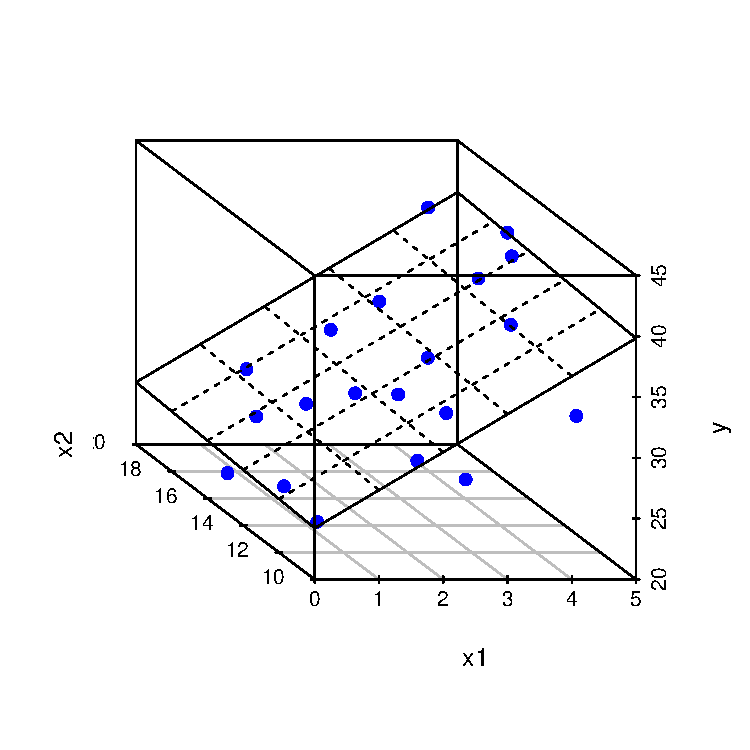
\includegraphics[width=0.6\linewidth]{figure/c1-1} 

\end{knitrout}

\end{frame}
%===============================================================================%


%===============================================================================%
\begin{frame}{Interpretação dos termos do modelo}

\begin{itemize}

\item $\beta _0$: intercepto da superfície de resposta. Valor de $Y$ quando  $X_{1} = X_2 = \dots X_{k=(p-1)} = 0$. Geralmente não tem um significado explícito. \pause
\vfill
\item $\beta _1$, $\beta _2$, \ldots, $\beta _k$: determinam o aumento em $E(Y)$ quando $X_{k}$ $(k=\{0,p-1\})$ aumenta em 1, e os demais $X_k$ permanecem constantes.\pause
\vfill
\item Cada coeficiente representa a contribuição absoluta de  $X_{k}$ para a estimativa de $E[Y]$ (ou $\beta _k = \frac{\delta E[Y]}{\delta X_{(k)}}$) \pause
\vfill
\item $\varepsilon _i$ continua sendo a diferença entre $Y_i$ e $E[Y_i]$

\end{itemize}

\end{frame}
%===============================================================================%

%===============================================================================%
\begin{frame}{Partição da variância}

A partição geral da variância segue o mesmo padrão do modelo simples, mas com diferentes graus de liberdade
\vfill
\resizebox{\textwidth}{!}{%
\begin{tabular}{lcllccc}
Fonte & GL & Soma Quadrados & Média Quadrados \\
\hline
& & & & & &\\
Regressão & $p-1$ & $SQ_{reg} = \mathbf{b'X'Y-\dfrac{1}{n} Y'JY}$ & $MQ_{reg} = \dfrac{SQ_{reg}}{p-1}$ \\[5ex]
Resíduos & $n-p$ & $SQ_{res} = \mathbf{Y'Y - b'X'Y}$ & $MQ_{res} = \dfrac{SQ_{res}}{n-p}$ \\[5ex]
Total & $n-1$ & $SQ_{tot} = \mathbf{Y'Y - \dfrac{1}{n} Y'JY}$ & $MQ_{tot} = \dfrac{SQ_{tot}}{n-1}$ \\[5ex]
\hline
\end{tabular}%
}

\end{frame}
%===============================================================================%


%===============================================================================%
\begin{frame}{Coeficiente de determinação múltiplo}

\begin{itemize}

\item O teste geral para a regressão ainda é feito usando $F^* = \frac{MS_{reg}}{MS_{res}}$, e a quantidade de variância explicada é representada por $R^2 = \frac{SQ_{reg}}{SQ_{tot}} = 1 - \frac{SQ_{erro}}{SQ_{tot}}$ \pause

\vfill

\item Quando novas variáveis são incluídas no modelo, $SQ_{res}$ permanece o mesmo ou diminui, mas nunca aumenta. \pause
\vfill
Por esse motivo, o $R^2$ aumenta mesmo que a quantidade de variância adicional explicada seja mínima. \pause
\vfill
\item Assim, não se pode confiar em $R^2$ como uma medida de qualidade do modelo (a interpretação de quantidade de variância explicada continua correta).


\end{itemize}

\end{frame}
%===============================================================================%


%===============================================================================%
\begin{frame}{Coeficiente de determinação múltiplo}

\begin{itemize}

\item O coeficiente de determinação ajustado ($R^2_a$) penaliza a razão de somas de quadrados pela razão entre os graus de liberdade:

\begin{equation*}
\centering
R^2_a = 1 - \left(\frac{n-1}{n-p}\right) \frac{SQ_{res}}{SQ_{tot}}
\end{equation*}

\pause
\item Dessa maneira, o ganho em explicação é ponderado pelo aumento de $\frac{(n-1)}{(n-p)}$, e o $R^2_a$ pode até diminuir com a adição de novas variáveis, se a contribuição não for importante.

\vfill

(Mas $R^2_a$ deixa de ter relação com \% de variância explicada)

\end{itemize}

\end{frame}
%===============================================================================%


%===============================================================================%
\begin{frame}{Inferências e Diagnósticos}

As inferências sobre o modelo (intervalos de confiança e testes de hipótese) seguem o mesmo modelo da regressão simples.

\vfill
As equações para estimativas dos erros são mais complexas, mas o princípio não se altera.

\end{frame}
%===============================================================================%


%===============================================================================%
\begin{frame}{Complicações adicionais}

Os modelos lineares de regressão múltipla apresentam algumas ``complicações'' a mais quando comparados com os modelos simples:
\vfill
\begin{itemize}

\item A existência de correlação entre as variáveis pode atrapalhar a nossa partição de variância (multicolinearidade).
\vfill
\item Os coeficientes $\beta$ normalmente não são diretamente comparáveis.
\vfill
\item Quando o número de variáveis independentes aumenta, a seleção final daquelas a serem inseridas no modelo torna-se mais difícil.
\vfill

\end{itemize}

\end{frame}
%===============================================================================%


%===============================================================================%
\begin{frame}{Multicolinearidade}

O modelo de regressão busca explicar parte da variância de $Y$ através da co-variância entre $Y$ e $X$ (partição de variâncias)
\vfill
Se as variáveis $X$ são independentes, cada porção da variância de $Y$ é explicada separadamente por cada $X$
\vfill
Mas se as variáveis preditoras foem correlacionadas, há redundância de informação, reduzindo a quantidade de informação disponívelpara estimação dos coeficientes $\beta$
\vfill


\end{frame}
%===============================================================================%


%===============================================================================%
\begin{frame}{Multicolinearidade}

Caso 1: $X_k$ perfeitamente independentes
\vfill
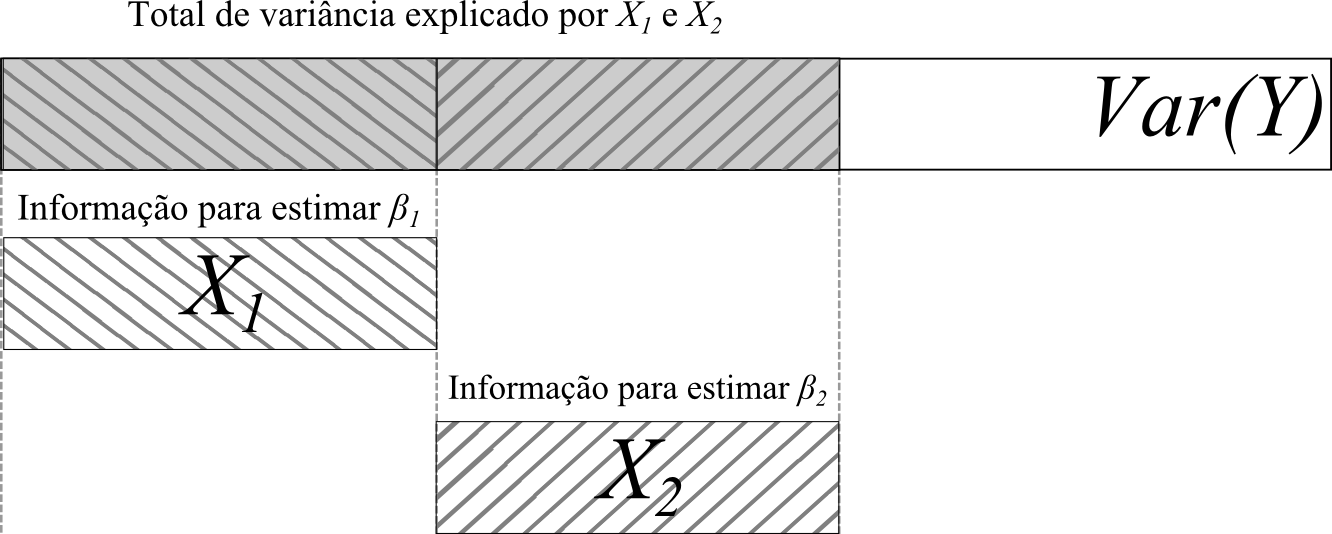
\includegraphics[width=1\textwidth]{multi1.png}


\end{frame}
%===============================================================================%


%===============================================================================%
\begin{frame}[fragile]{Multicolinearidade}

Caso 1: $X_k$ perfeitamente independentes
\vfill
Nesse caso, a contribuição de $X_1$ e $X_2$ são exatamente as mesmas de dois modelos lineares simples:
\vfill
\begin{knitrout}\tiny
\definecolor{shadecolor}{rgb}{0.969, 0.969, 0.969}\color{fgcolor}\begin{kframe}
\begin{alltt}
\hlstd{x1} \hlkwb{<-} \hlkwd{c}\hlstd{(}\hlnum{4}\hlstd{,}\hlnum{4}\hlstd{,}\hlnum{4}\hlstd{,}\hlnum{4}\hlstd{,}\hlnum{6}\hlstd{,}\hlnum{6}\hlstd{,}\hlnum{6}\hlstd{,}\hlnum{6}\hlstd{)}
\hlstd{x2} \hlkwb{<-} \hlkwd{c}\hlstd{(}\hlnum{2}\hlstd{,}\hlnum{2}\hlstd{,}\hlnum{3}\hlstd{,}\hlnum{3}\hlstd{,}\hlnum{2}\hlstd{,}\hlnum{2}\hlstd{,}\hlnum{3}\hlstd{,}\hlnum{3}\hlstd{)}
\hlstd{y} \hlkwb{<-} \hlkwd{c}\hlstd{(}\hlnum{42}\hlstd{,}\hlnum{39}\hlstd{,}\hlnum{48}\hlstd{,}\hlnum{51}\hlstd{,}\hlnum{49}\hlstd{,}\hlnum{53}\hlstd{,}\hlnum{61}\hlstd{,}\hlnum{60}\hlstd{)}

\hlkwd{cor}\hlstd{(x1,x2)}
\end{alltt}
\begin{verbatim}
## [1] 0
\end{verbatim}
\end{kframe}
\end{knitrout}

\end{frame}
%===============================================================================%


%===============================================================================%
\begin{frame}[fragile]{Multicolinearidade}

Caso 1: $X_k$ perfeitamente independentes
\vfill

\begin{knitrout}\tiny
\definecolor{shadecolor}{rgb}{0.969, 0.969, 0.969}\color{fgcolor}\begin{kframe}
\begin{alltt}
\hlstd{m1} \hlkwb{<-} \hlkwd{lm}\hlstd{(y} \hlopt{~} \hlstd{x1);m1}
\end{alltt}
\begin{verbatim}
## 
## Call:
## lm(formula = y ~ x1)
## 
## Coefficients:
## (Intercept)           x1  
##      23.500        5.375
\end{verbatim}
\begin{alltt}
\hlkwd{anova}\hlstd{(m1)}
\end{alltt}
\begin{verbatim}
## Analysis of Variance Table
## 
## Response: y
##           Df Sum Sq Mean Sq F value
## x1         1 231.12 231.125   7.347
## Residuals  6 188.75  31.458        
##            Pr(>F)  
## x1        0.03508 *
## Residuals          
## ---
## Signif. codes:  
##   0 '***' 0.001 '**' 0.01 '*' 0.05
##   '.' 0.1 ' ' 1
\end{verbatim}
\end{kframe}
\end{knitrout}

\end{frame}
%===============================================================================%



%===============================================================================%
\begin{frame}[fragile]{Multicolinearidade}

Caso 1: $X_k$ perfeitamente independentes
\vfill

\begin{knitrout}\tiny
\definecolor{shadecolor}{rgb}{0.969, 0.969, 0.969}\color{fgcolor}\begin{kframe}
\begin{alltt}
\hlstd{m2} \hlkwb{<-} \hlkwd{lm}\hlstd{(y} \hlopt{~} \hlstd{x2); m2}
\end{alltt}
\begin{verbatim}
## 
## Call:
## lm(formula = y ~ x2)
## 
## Coefficients:
## (Intercept)           x2  
##       27.25         9.25
\end{verbatim}
\begin{alltt}
\hlkwd{anova}\hlstd{(m2)}
\end{alltt}
\begin{verbatim}
## Analysis of Variance Table
## 
## Response: y
##           Df Sum Sq Mean Sq F value
## x2         1 171.12 171.125  4.1276
## Residuals  6 248.75  41.458        
##            Pr(>F)  
## x2        0.08846 .
## Residuals          
## ---
## Signif. codes:  
##   0 '***' 0.001 '**' 0.01 '*' 0.05
##   '.' 0.1 ' ' 1
\end{verbatim}
\end{kframe}
\end{knitrout}

\end{frame}
%===============================================================================%


%===============================================================================%
\begin{frame}[fragile]{Multicolinearidade}

Caso 1: $X_k$ perfeitamente independentes
\vfill

\begin{knitrout}\tiny
\definecolor{shadecolor}{rgb}{0.969, 0.969, 0.969}\color{fgcolor}\begin{kframe}
\begin{alltt}
\hlstd{m3} \hlkwb{<-} \hlkwd{lm}\hlstd{(y} \hlopt{~} \hlstd{x1} \hlopt{+} \hlstd{x2); m3}
\end{alltt}
\begin{verbatim}
## 
## Call:
## lm(formula = y ~ x1 + x2)
## 
## Coefficients:
## (Intercept)           x1           x2  
##       0.375        5.375        9.250
\end{verbatim}
\begin{alltt}
\hlkwd{anova}\hlstd{(m3)}
\end{alltt}
\begin{verbatim}
## Analysis of Variance Table
## 
## Response: y
##           Df  Sum Sq Mean Sq F value
## x1         1 231.125 231.125  65.567
## x2         1 171.125 171.125  48.546
## Residuals  5  17.625   3.525        
##              Pr(>F)    
## x1        0.0004657 ***
## x2        0.0009366 ***
## Residuals              
## ---
## Signif. codes:  
##   0 '***' 0.001 '**' 0.01 '*' 0.05
##   '.' 0.1 ' ' 1
\end{verbatim}
\end{kframe}
\end{knitrout}

\end{frame}
%===============================================================================%



%===============================================================================%
\begin{frame}{Multicolinearidade}
 
Caso 2: $X_k$ perfeitamente correlacionados
\vfill
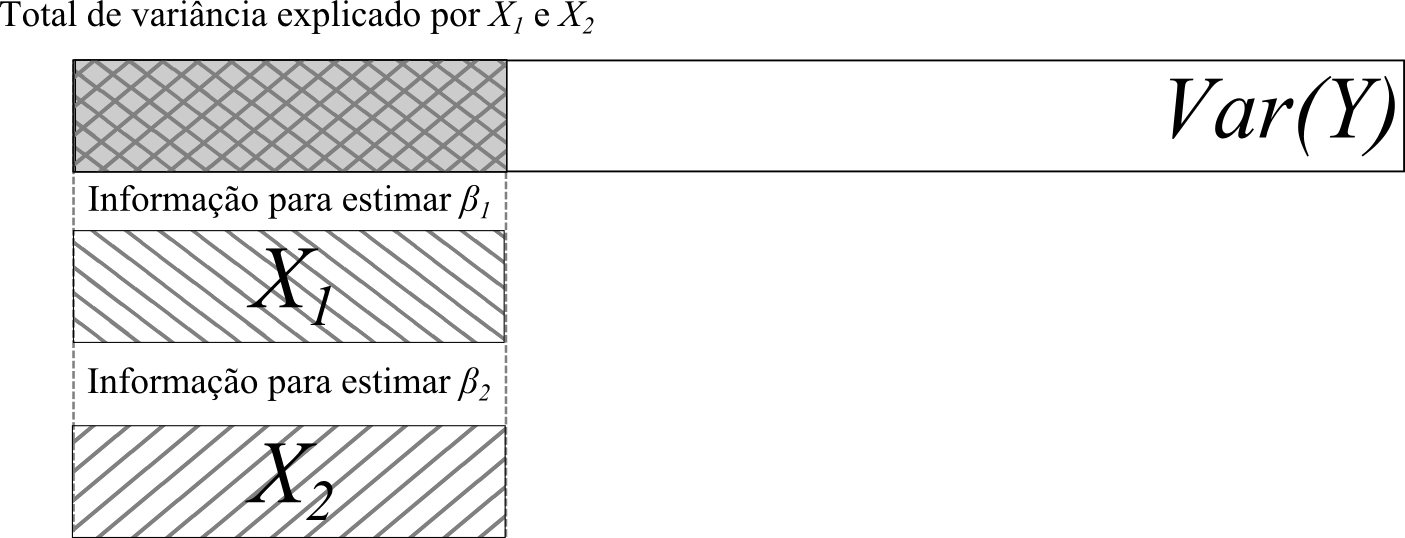
\includegraphics[width=1\textwidth]{multi3.png}

\end{frame}
%===============================================================================%

%===============================================================================%
\begin{frame}[fragile]{Multicolinearidade}

Caso 2: $X_k$ perfeitamente correlacionados
\vfill
Nesse caso, não há variância restante para estimar $\beta _2$ após a estimação de $\beta _1$:
\vfill
\begin{knitrout}\tiny
\definecolor{shadecolor}{rgb}{0.969, 0.969, 0.969}\color{fgcolor}\begin{kframe}
\begin{alltt}
\hlstd{x1} \hlkwb{<-} \hlkwd{c}\hlstd{(}\hlnum{4}\hlstd{,}\hlnum{4}\hlstd{,}\hlnum{4}\hlstd{,}\hlnum{4}\hlstd{,}\hlnum{6}\hlstd{,}\hlnum{6}\hlstd{,}\hlnum{6}\hlstd{,}\hlnum{6}\hlstd{)}
\hlstd{x2} \hlkwb{<-} \hlstd{x1}
\hlstd{y} \hlkwb{<-} \hlkwd{c}\hlstd{(}\hlnum{42}\hlstd{,}\hlnum{39}\hlstd{,}\hlnum{48}\hlstd{,}\hlnum{51}\hlstd{,}\hlnum{49}\hlstd{,}\hlnum{53}\hlstd{,}\hlnum{61}\hlstd{,}\hlnum{60}\hlstd{)}

\hlkwd{cor}\hlstd{(x1,x2)}
\end{alltt}
\begin{verbatim}
## [1] 1
\end{verbatim}
\end{kframe}
\end{knitrout}

\end{frame}
%===============================================================================%


%===============================================================================%
\begin{frame}[fragile]{Multicolinearidade}

Caso 2: $X_k$ perfeitamente correlacionados
\vfill

\begin{knitrout}\tiny
\definecolor{shadecolor}{rgb}{0.969, 0.969, 0.969}\color{fgcolor}\begin{kframe}
\begin{alltt}
\hlstd{m1} \hlkwb{<-} \hlkwd{lm}\hlstd{(y} \hlopt{~} \hlstd{x1} \hlopt{+} \hlstd{x2); m1}
\end{alltt}
\begin{verbatim}
## 
## Call:
## lm(formula = y ~ x1 + x2)
## 
## Coefficients:
## (Intercept)           x1           x2  
##      23.500        5.375           NA
\end{verbatim}
\begin{alltt}
\hlkwd{anova}\hlstd{(m1)}
\end{alltt}
\begin{verbatim}
## Analysis of Variance Table
## 
## Response: y
##           Df Sum Sq Mean Sq F value
## x1         1 231.12 231.125   7.347
## Residuals  6 188.75  31.458        
##            Pr(>F)  
## x1        0.03508 *
## Residuals          
## ---
## Signif. codes:  
##   0 '***' 0.001 '**' 0.01 '*' 0.05
##   '.' 0.1 ' ' 1
\end{verbatim}
\end{kframe}
\end{knitrout}

\end{frame}
%===============================================================================%

%===============================================================================%
\begin{frame}[fragile]{Multicolinearidade}

Caso 2: $X_k$ perfeitamente correlacionados
\vfill

\begin{knitrout}\tiny
\definecolor{shadecolor}{rgb}{0.969, 0.969, 0.969}\color{fgcolor}\begin{kframe}
\begin{alltt}
\hlstd{m2} \hlkwb{<-} \hlkwd{lm}\hlstd{(y} \hlopt{~} \hlstd{x2} \hlopt{+} \hlstd{x1); m2}
\end{alltt}
\begin{verbatim}
## 
## Call:
## lm(formula = y ~ x2 + x1)
## 
## Coefficients:
## (Intercept)           x2           x1  
##      23.500        5.375           NA
\end{verbatim}
\begin{alltt}
\hlkwd{anova}\hlstd{(m2)}
\end{alltt}
\begin{verbatim}
## Analysis of Variance Table
## 
## Response: y
##           Df Sum Sq Mean Sq F value
## x2         1 231.12 231.125   7.347
## Residuals  6 188.75  31.458        
##            Pr(>F)  
## x2        0.03508 *
## Residuals          
## ---
## Signif. codes:  
##   0 '***' 0.001 '**' 0.01 '*' 0.05
##   '.' 0.1 ' ' 1
\end{verbatim}
\end{kframe}
\end{knitrout}

\end{frame}
%===============================================================================%


%===============================================================================%
\begin{frame}{Multicolinearidade}

Caso 3: $X_k$ parcialmente correlacionados
\vfill
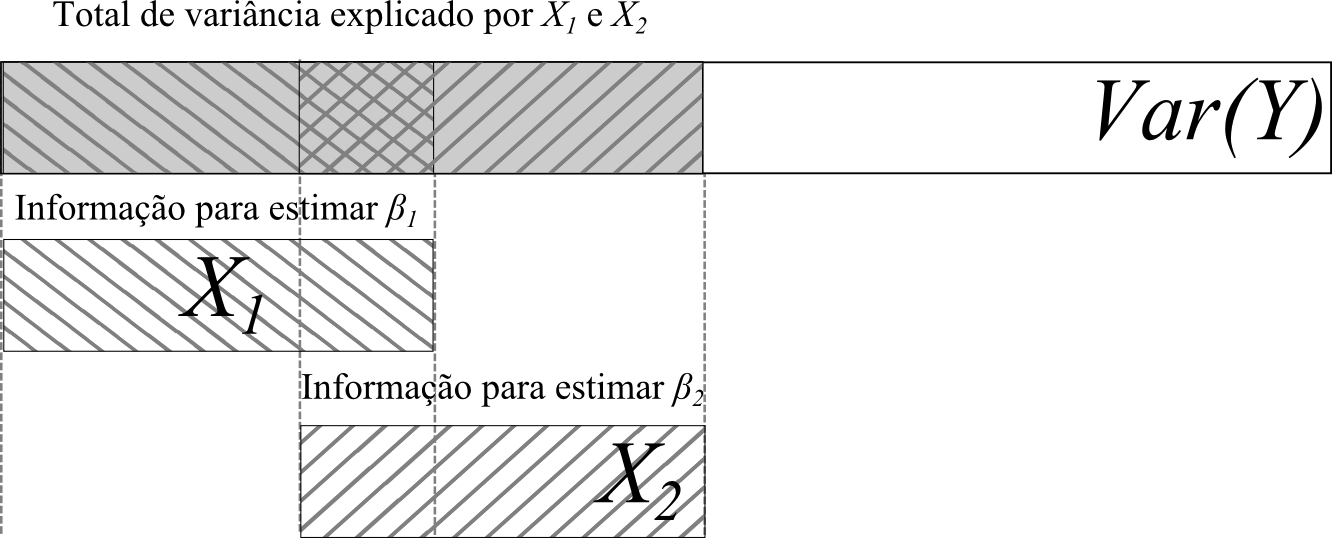
\includegraphics[width=1\textwidth]{multi2.png}
 
\end{frame}
%===============================================================================%


%===============================================================================%
\begin{frame}[fragile]{Multicolinearidade}

Caso 3: $X_k$ parcialmente correlacionados
\vfill
Nesse caso, há "menos" variância restante para estimar $\beta _2$ após a estimação de $\beta _1$:
\vfill
\begin{knitrout}\tiny
\definecolor{shadecolor}{rgb}{0.969, 0.969, 0.969}\color{fgcolor}\begin{kframe}
\begin{alltt}
\hlstd{x1} \hlkwb{<-} \hlkwd{c}\hlstd{(}\hlnum{4}\hlstd{,}\hlnum{4}\hlstd{,}\hlnum{4}\hlstd{,}\hlnum{4}\hlstd{,}\hlnum{6}\hlstd{,}\hlnum{6}\hlstd{,}\hlnum{6}\hlstd{,}\hlnum{6}\hlstd{)}
\hlkwd{set.seed}\hlstd{(}\hlnum{154}\hlstd{)}
\hlstd{x2} \hlkwb{<-} \hlstd{x1} \hlopt{+} \hlkwd{runif}\hlstd{(}\hlnum{8}\hlstd{,}\hlnum{0}\hlstd{,}\hlnum{1}\hlstd{)}
\hlstd{y} \hlkwb{<-} \hlkwd{c}\hlstd{(}\hlnum{42}\hlstd{,}\hlnum{39}\hlstd{,}\hlnum{48}\hlstd{,}\hlnum{51}\hlstd{,}\hlnum{49}\hlstd{,}\hlnum{53}\hlstd{,}\hlnum{61}\hlstd{,}\hlnum{60}\hlstd{)}

\hlkwd{cor}\hlstd{(x1,x2)}
\end{alltt}
\begin{verbatim}
## [1] 0.9592065
\end{verbatim}
\end{kframe}
\end{knitrout}

\end{frame}
%===============================================================================%


%===============================================================================%
\begin{frame}[fragile]{Multicolinearidade}

Caso 3: $X_k$ parcialmente correlacionados
\vfill

\begin{knitrout}\tiny
\definecolor{shadecolor}{rgb}{0.969, 0.969, 0.969}\color{fgcolor}\begin{kframe}
\begin{alltt}
\hlstd{m1} \hlkwb{<-} \hlkwd{lm}\hlstd{(y} \hlopt{~} \hlstd{x1} \hlopt{+} \hlstd{x2); m1}
\end{alltt}
\begin{verbatim}
## 
## Call:
## lm(formula = y ~ x1 + x2)
## 
## Coefficients:
## (Intercept)           x1           x2  
##      23.886        6.878       -1.418
\end{verbatim}
\begin{alltt}
\hlkwd{anova}\hlstd{(m1)}
\end{alltt}
\begin{verbatim}
## Analysis of Variance Table
## 
## Response: y
##           Df Sum Sq Mean Sq F value
## x1         1 231.12 231.125  6.1739
## x2         1   1.57   1.570  0.0419
## Residuals  5 187.18  37.436        
##            Pr(>F)  
## x1        0.05552 .
## x2        0.84583  
## Residuals          
## ---
## Signif. codes:  
##   0 '***' 0.001 '**' 0.01 '*' 0.05
##   '.' 0.1 ' ' 1
\end{verbatim}
\end{kframe}
\end{knitrout}

\end{frame}
%===============================================================================%

%===============================================================================%
\begin{frame}[fragile]{Multicolinearidade}

Caso 3: $X_k$ parcialmente correlacionados
\vfill

\begin{knitrout}\tiny
\definecolor{shadecolor}{rgb}{0.969, 0.969, 0.969}\color{fgcolor}\begin{kframe}
\begin{alltt}
\hlstd{m2} \hlkwb{<-} \hlkwd{lm}\hlstd{(y} \hlopt{~} \hlstd{x2} \hlopt{+} \hlstd{x1); m2}
\end{alltt}
\begin{verbatim}
## 
## Call:
## lm(formula = y ~ x2 + x1)
## 
## Coefficients:
## (Intercept)           x2           x1  
##      23.886       -1.418        6.878
\end{verbatim}
\begin{alltt}
\hlkwd{anova}\hlstd{(m2)}
\end{alltt}
\begin{verbatim}
## Analysis of Variance Table
## 
## Response: y
##           Df  Sum Sq Mean Sq F value
## x2         1 202.448 202.448  5.4078
## x1         1  30.246  30.246  0.8080
## Residuals  5 187.180  37.436        
##            Pr(>F)  
## x2        0.06759 .
## x1        0.40992  
## Residuals          
## ---
## Signif. codes:  
##   0 '***' 0.001 '**' 0.01 '*' 0.05
##   '.' 0.1 ' ' 1
\end{verbatim}
\end{kframe}
\end{knitrout}

\end{frame}
%===============================================================================%



%===============================================================================%
\begin{frame}{Multicolinearidade}

Que parte do modelo de regressão esperamos que vá ser afetada pela multicolinearidade?  \pause

\begin{itemize}

\item Os coeficientes $\beta _1$, \ldots, $\beta _k$ \pause

\end{itemize}

Qual será o principal efeito da multicolinearidade sobre a especificação do modelo? \pause

\begin{itemize}

\item As propriedades dos estimadores não se alteram (\emph{BLUE}) \pause

\item Devido à redução na quantidade de informação disponível, o erro na estimaçãode cada $b_k$ aumenta. \pause

\item Como a informação é redundante, múltiplas combinações de $X_k$ e $b_k$ podem dar o mesmo resultado final. 
 
\end{itemize}

\end{frame}
%===============================================================================%



\end{document}
